\chapter{Industry Practice} % Main chapter title

\label{Chapter9} % Change X to a consecutive number; for referencing this chapter elsewhere, use \ref{ChapterX}

\lhead{Chapter 9. \emph{Industry Practice}} % Change X to a consecutive number; this is for the header on each page - perhaps a shortened title


%----------------------------------------------------------------------------------------
%	CHAPTER INTRO
%----------------------------------------------------------------------------------------
    
This chapter reports lived experiences in collaboration and communication gathered from industry through questionnaires and follow-up interviews.


%----------------------------------------------------------------------------------------
%	SECTION 1
%----------------------------------------------------------------------------------------

\section{Questionnaire Responses}

% A questionnaire was designed using Google Forms and distributed to the researcher's and her supervisor's relevant contacts in the construction industry (see questionnaire in appendix \ref{questionnaire}).


%------------------------------
%	SUBSECTION 1
%------------------------------

\subsection{Background}

The sample size of the survey was 40.
Most of the respondents consisted of consulting engineers, but there were also contractors, BIM managers or coordinators, policy and regulation consultants, construction product manufacturers, project managers and site architects (see Figure \ref{positions}).
Due to the uneven representation of occupations causing the data to be skewed, it has been decided to use count as opposed to percentage in the charts that compare certain variables among the respondents' occupations.

\begin{figure}[htbp]
	\centering
	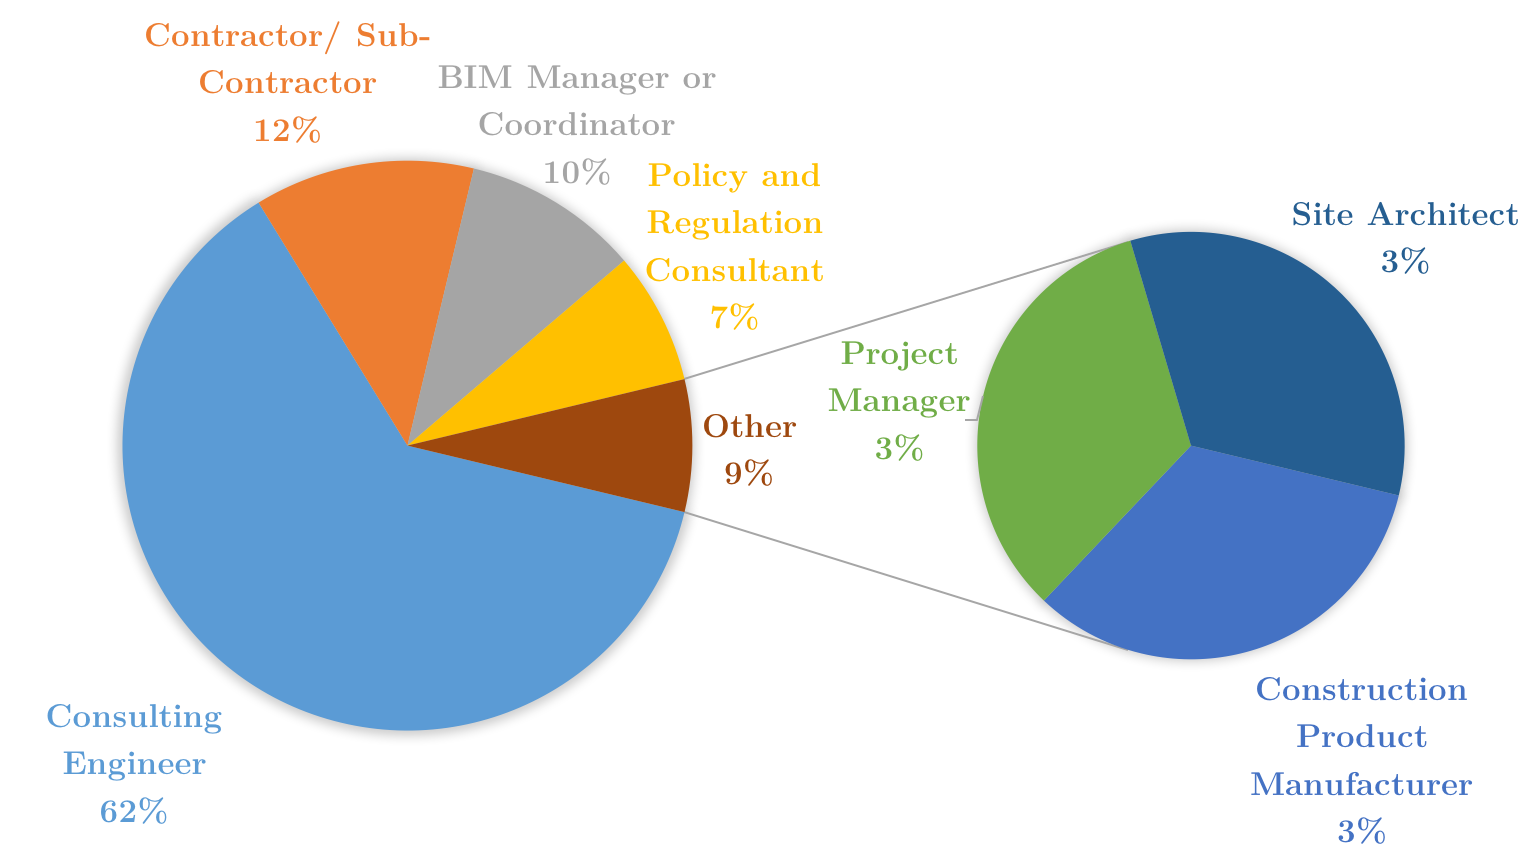
\includegraphics[width=\textwidth]{figures/positions.png}
	\rule{\textwidth}{0.5pt} % use line???
	\caption{Occupations of the survey respondents.}
	\label{positions}
\end{figure}


% Count has been used instead of percentage in certain graphs due to skewed responses…

90\% of the respondents work or have worked in building services, 79\% of whom were involved in one or more of the MEP fields (see Figure \ref{bs_fields}).
The respondents ranged in their number of years of experience in building services, from 0-5 years to more than 35 years (see Figure \ref{bs_yrs}).
Some of the respondents that have not directly worked in building services sometimes oversee or coordinate work by building services engineers.

% EXPANDED PIE CHART
\begin{figure}[htbp]
	\centering
	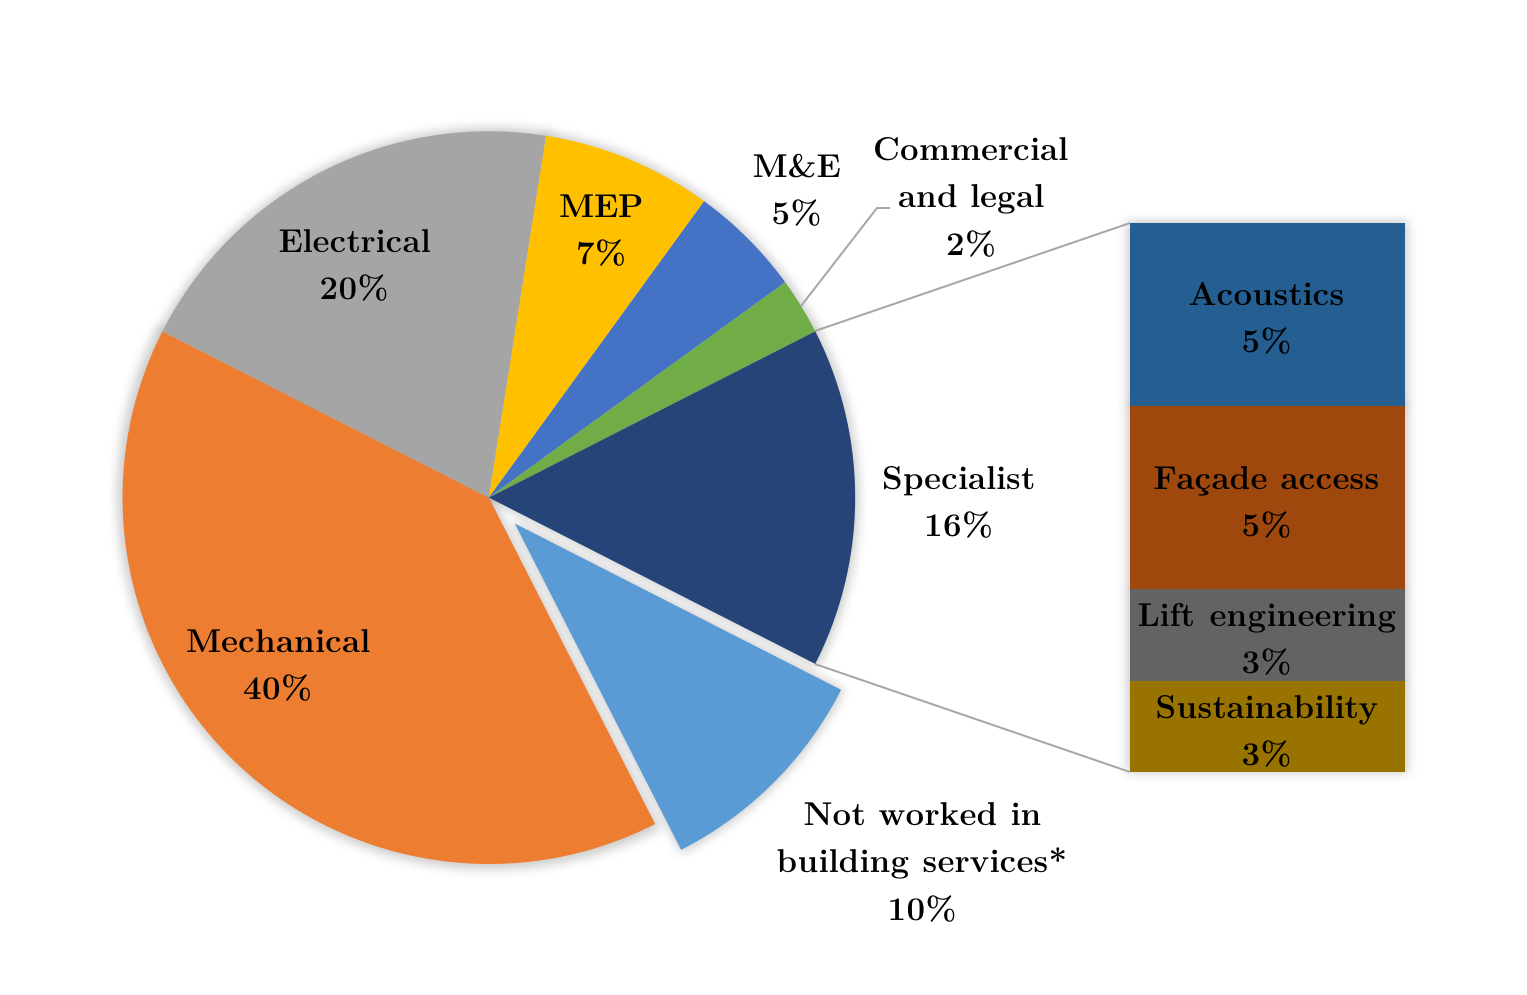
\includegraphics[width=\textwidth]{figures/BS-fields.png}
	\rule{\textwidth}{0.5pt} % use line???
	\caption[Building services fields of respondents.]{Building services fields of respondents. (*Some of these respondents either oversee work by building services engineers or coordinate between architectural, structural and MEP work.)}
	\label{bs_fields}
\end{figure}



% BAR CHART
\begin{figure}[htbp]
	\centering
	
\includegraphics[width=\textwidth]{figures/Yrs-in-BS.eps}
	\rule{\textwidth}{0.5pt} % use line???
	\caption[Respondents' years working in building services.]{Respondents' years working in building services. (*These respondents have not worked in building services, but some of them either oversee work by building services engineers or coordinate between architectural, structural and MEP work.)}
	\label{bs_yrs}
\end{figure}

The respondents ranged in the number of years they had worked with BIM, from no experience to at least eight years' experience (see Figure \ref{bim_yrs}).
They also ranged in their confidence in working with BIM, with 43.6\% of the respondents considering themselves BIM literate, 38.5\% BIM illiterate, and 18\% neither nor (see Figure \ref{bim_literacy}).
% SPSS has been updated with currently 40 entries
It should be noted that the questionnaire did not define what was meant by `BIM literacy'.
Since BIM is an innovation in both technology and process, the respondents may have interpreted `BIM literacy' as their familiarity with either the technology, the process, or both.
Hence, the BIM literacy responses may be ambiguous.

As seen in Figure \ref{bim_literacy_X_bim_yrs}, there appears to be a correlation between the respondents' years of working with BIM and their BIM literacy.
100\% of the respondents that have worked with BIM for at least eight years and about 70\% of those that have worked with BIM for 3-7 years considered themselves BIM literate.
The responses of those with less or no experience in BIM peak at `Disagree'.
Interestingly, 30\% of those with less than two years' BIM experience and 12\% of those with no BIM experience considered themselves BIM literate.
% Perhaps they find themselves literate in BIM processes, as opposed to the technology.
% N.B. The questionnaire wasn't clear on what BIM literacy means and did not distinguish the BIM technology from the BIM process.

% BAR CHART
\begin{figure}[htbp]
	\centering
	
\includegraphics[width=\textwidth]{figures/BIM_yrs.eps}
	\rule{\textwidth}{0.5pt} % use line???
	\caption{Respondents' years working with BIM.}
	\label{bim_yrs}
\end{figure}


% BAR CHART
\begin{figure}[htbp]
	\centering
	
\includegraphics[width=\textwidth]{figures/BIM-literacy.eps}
	\rule{\textwidth}{0.5pt} % use line???
	\caption[Respondents' BIM literacy.]{Responses to the question ``How much do you agree with the statement `I am BIM literate'?".}
	\label{bim_literacy}
\end{figure}




% BAR CHART
\begin{figure}[htbp]
	\centering
	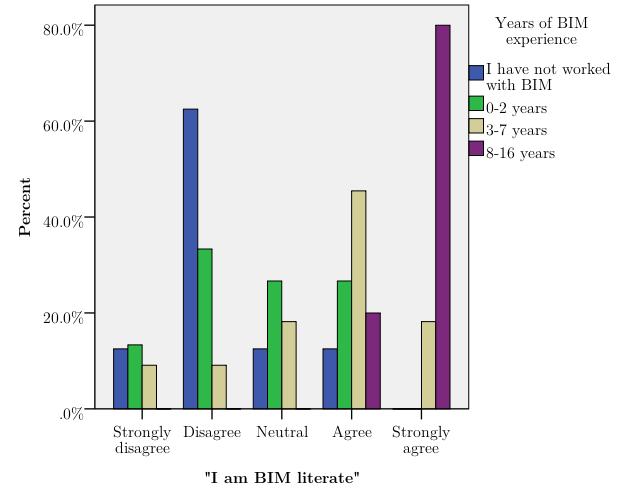
\includegraphics[width=0.9\textwidth]{figures/BIM_literacy_X_BIM_yrs.png}
	\rule{0.9\textwidth}{0.5pt} % use line???
	\caption{Respondents' years of BIM experience in terms of their BIM literacy.}
	\label{bim_literacy_X_bim_yrs}
\end{figure}

According to Figure \ref{bim_training_X_bim_literacy},
% compares the respondents' BIM literacy with their training in BIM.
there also appears to be a correlation between the respondents' BIM training and their BIM literacy.
Those with no or limited BIM experience are less confident in BIM.
BIM literacy ranges from illiterate to literate among the self-taught and those who received BIM training at the workplace.
Furthermore, it seems that people who are formally trained in BIM at university or college have greater confidence in their BIM abilities, but their sample size in this survey is too small to be sure.
% However, the sample size of people received BIM training at university or college was 
% There was also a range of BIM literacy responses depending on where respondents learned BIM.
% i.e. there is no correlation between BIM literacy and place of BIM training as far as we can tell.

% BAR CHART
\begin{figure}[htbp]
	\centering
	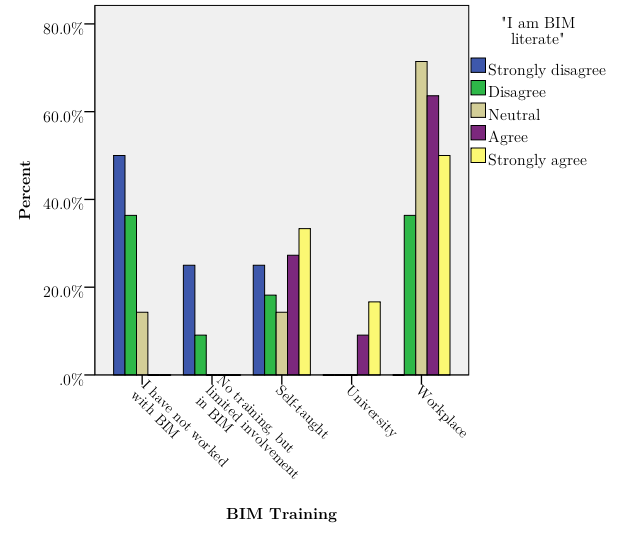
\includegraphics[width=0.9\textwidth]{figures/BIM_trainingXliteracy.png}
	\rule{0.9\textwidth}{0.5pt} % use line???
	\caption{Respondents' BIM literacy in terms of their BIM training.}
	\label{bim_training_X_bim_literacy}
\end{figure}

Figure \ref{position_X_bim_literacy} displays the respondents' BIM literacy in terms of their occupation.
As expected, 100\% of the BIM managers and coordinators considered themselves BIM literate.
Interestingly, there appears to be a wide range of BIM literacy among consulting engineers.
Figure \ref{consulting_X_bim_literacy} looks more closely at the consulting engineers' BIM literacy.
% Looking more closely at consulting engineers (them being our majority and focal point), 
None of the consulting engineers strongly agreed to being BIM literate.
Only 28\% considered themselves BIM literate, and almost 50\% considered themselves illiterate.


% BAR CHART
\begin{figure}[htbp]
	\centering
	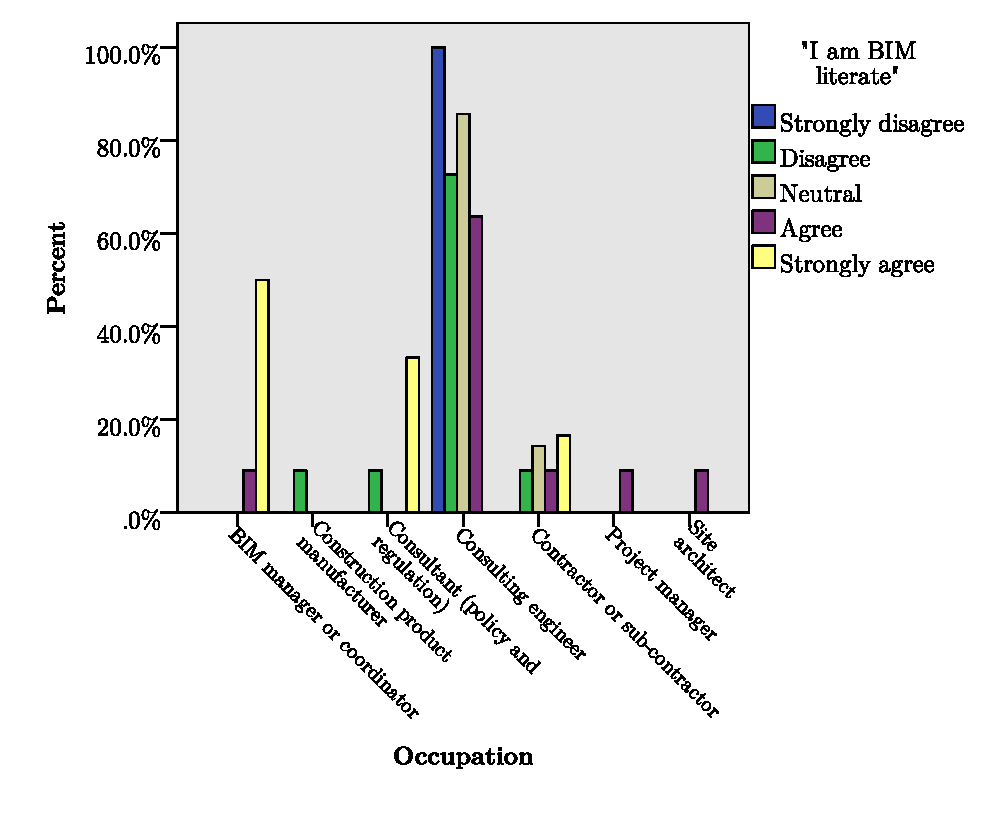
\includegraphics[width=0.9\textwidth]{figures/BIMLiteracyXPositions.eps}
	\rule{0.9\textwidth}{0.5pt} % use line???
	\caption{Respondents' BIM literacy in terms of their occupation.}
	\label{position_X_bim_literacy}
\end{figure}


% BAR CHART
\begin{figure}[htbp]
	\centering
	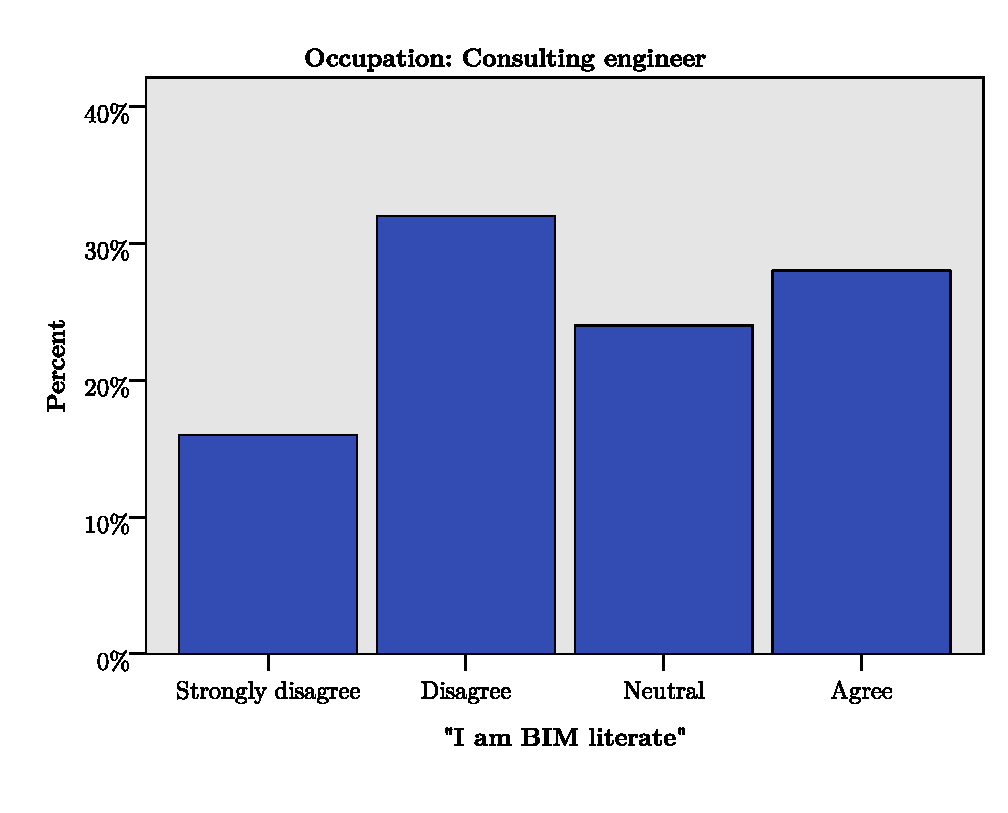
\includegraphics[width=0.9\textwidth]{figures/consultingXbimliteracy1.eps}
	\rule{0.9\textwidth}{0.5pt} % use line???
	\caption{Consulting engineers' BIM literacy.}
	\label{consulting_X_bim_literacy}
\end{figure}


%------------------------------
%	SUBSECTION 2
%------------------------------

\subsection{Contractors Only}

Only five of the respondents were contractors or sub-contractors.
All of these contractors have worked in building services for at least 16 years in either mechanical, or electrical, or both fields.
One of these contractors never receives Stage 4 BIM models from consultants, and another said that they were \say{not involved to that extent}.

Out of the remaining three contractors, two said that they typically receive generic and not necessarily coordinated Stage 4 models from consultants, and one said that they typically receive specific and spatially coordinated models.
One of the contractors that receives generic models typically finds that the models' intelligence breaks down when they replace generic objects with specific objects.
The other two do not seem to encounter this problem.

All three contractors typically re-build the consultant's BIM model.
They do this in spite of whether the model is specific and spatially coordinated to begin with, and in spite of not encountering BIM model breakdowns.
% So, why then do they do this?
% Is it not an unnecessary surplus of time and effort?

Finally, of the three contractors, only two send models to workshops for automatic fabrication of parts.
However, one of these respondents specified that they do this activity at Stage 5, not 4.

\begin{comment}
The two contractors that typically receive generic models have agreed to participate in an interview.
It would be interesting to speak with both of them, considering that:
\begin{itemize}
    \item They both have different experiences with model intelligence breaking down
    \item They both re-build models
    \item They both send out models to workshops for automatic fabrication of parts
\end{itemize}
\end{comment}


%------------------------------
%	SUBSECTION 3
%------------------------------

\subsection{Work Stage Deliverables}

The respondents were asked about their understanding of expected work stage deliverables.
This was done to verify whether there might indeed be a need to clarify MEP consultants' work stage deliverables, as \cite{Quigley2017} indicated.
% Therefore, this may contradict with what \cite{Quigley2017} said about there being a need to clarify what consulting MEP engineers need to deliver at each work stage.
88\% of the consulting engineers agreed or strongly agreed that they generally understand the level of information they are expected to deliver at the end of every work stage (see Figure \ref{consulting_X_understanding}).
8\% disagreed and 4\% were neutral.
One of those who disagreed, an experienced building services consulting engineer, explained that, \say{There is a lot of nonsense talked about BIM and poor specification of what is expected by those writing the contracts.}
One of those who responded neutrally, a building services consulting engineer with 6-15 years experience, explained that they \say{have an idea, but not the detail}.
One of those who agreed, an experienced building services consulting engineer, noted that they have an interpretation of what they believe each stage should look like, but that they \say{doubt if clients, contractors, etc… would agree as [it] is not set in stone as of yet}.

% BAR CHART
\begin{figure}[htbp]
	\centering
	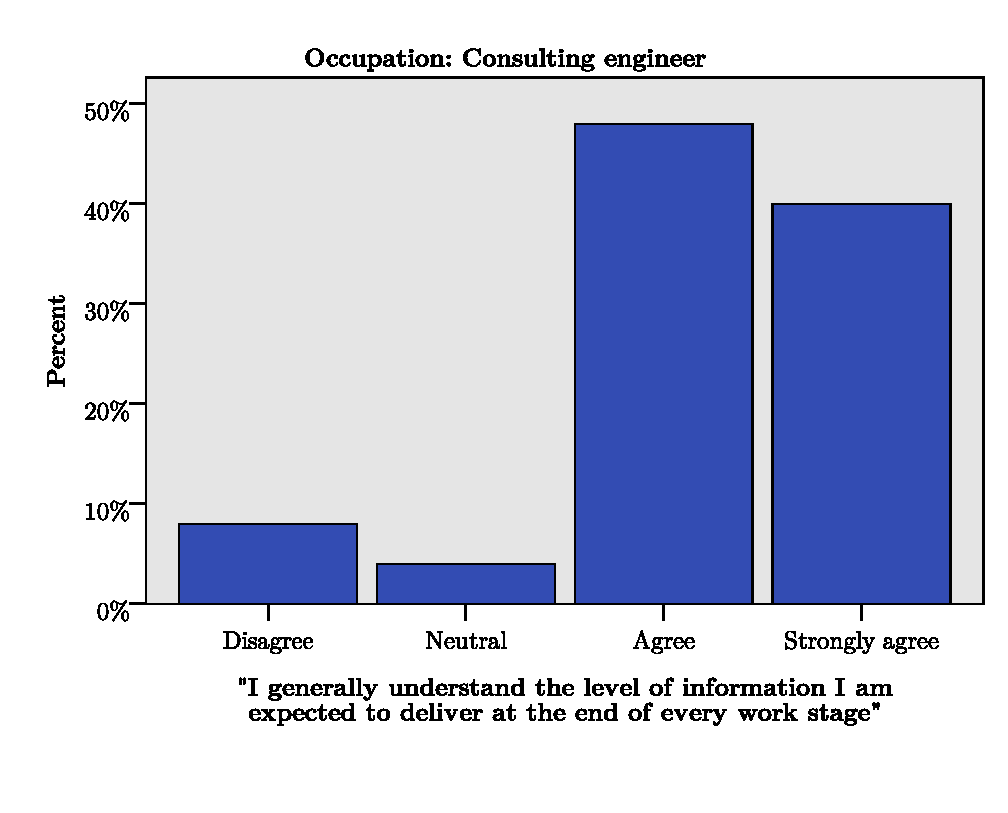
\includegraphics[width=0.9\textwidth]{figures/ConsultingXUnderstanding.eps}
	\rule{0.9\textwidth}{0.5pt} % use line???
	\caption{Consulting engineers' understanding of expected deliverables at the end of every work stage}
	\label{consulting_X_understanding}
\end{figure}


From an outside perspective, a project manager says the following: \say{I ordinarily am involved with setting the level that M\&E consultants are to deliver rather than delivering myself.  I generally find that M\&E consultants do understand what is required, but sometimes they resist delivering a high level of detail at early stages as they prefer to leave the detailed design to be done by sub-contractors}.
Our results (with 88\% consulting engineers agreeing to understand the work stage deliverables) reflect the project manager's observation of M\&E consultants generally understanding what is required.



%------------------------------
%	SUBSECTION 4
%------------------------------

\subsection{Levels of Definition}

The majority (60\%) of the respondents were familiar with the term LOD (see Figure \ref{LODfam}), whereas 17.5\% had never heard of the term.
The majority (56\%) of the consulting engineers, however, had either never heard of the term or were aware but not familiar with it.

% BAR CHART in count
\begin{figure}[htbp]
	\centering
	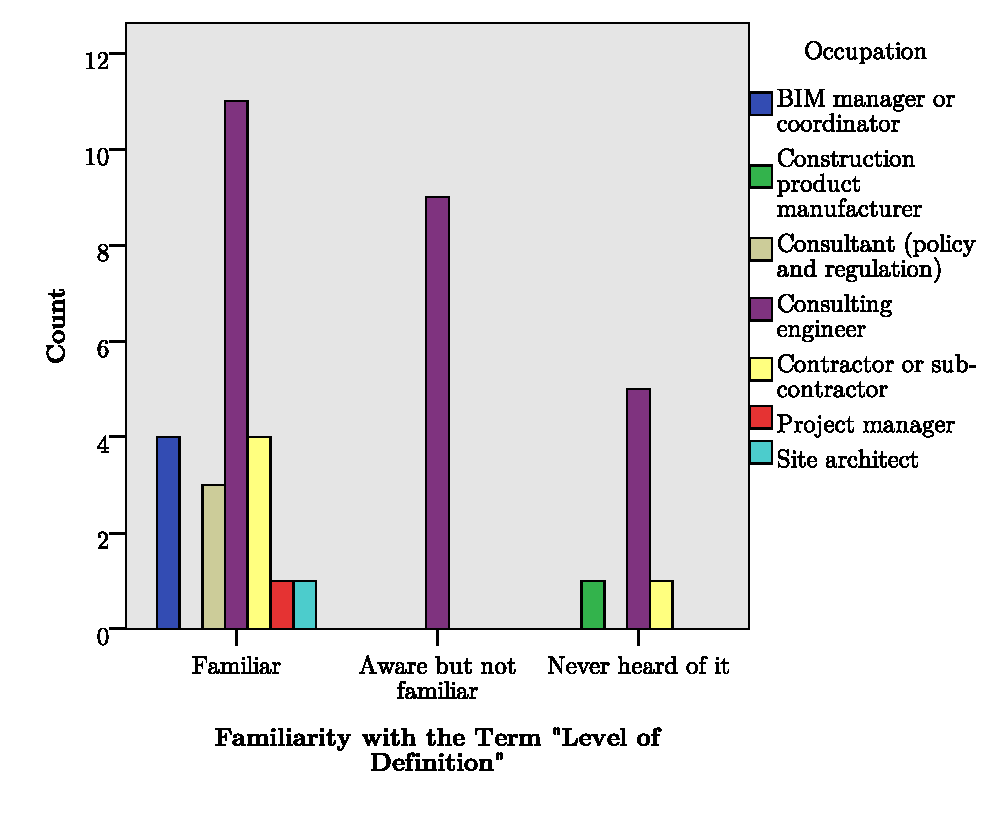
\includegraphics[width=0.9\textwidth]{figures/OccupationXLodCount.eps}
	\rule{0.9\textwidth}{0.5pt} % use line???
	\caption{Respondents' occupations in terms of their familiarity with the term LOD.}
	\label{LODfam}
\end{figure}


90\% and 92.5\% of the respondents accurately matched the term LoD with graphical content and the term LoI with non-graphical content, respectively (see Figure \ref{lod_loi}).
This can be seen as a positive outcome.
Despite 40\% of the respondents not being familiar with the term LOD, most of the respondents correctly matched the terms and definitions.
This may imply that LoD and LoI are fitting terms to indicate the amounts of graphical and non-graphical content in BIM models.
% It should be noted that the terms may \say{give themselves away} by their somewhat descriptiveness (for example, \say{level of \emph{information}} suits non-graphical content better than it does graphical), but that just goes to say that they are good names.

% BAR CHART in count???
\begin{figure}[htbp]
	\centering
	
\includegraphics[width=0.9\textwidth]{figures/lod_loi.eps}
	\rule{0.9\textwidth}{0.5pt} % use line???
	\caption{Respondents' LoD and LoI term-and-definition matches.}
	\label{lod_loi}
\end{figure}


The open-ended question \say{Have you noticed a difference in levels of definition from one project to the next? If so, please describe,} received the most attention out of the five open-ended questions provided throughout the questionnaire, with responses from 52.5\% (21) of the respondents.

5\% (9.5\% of 21) of the respondents 
indicated that LODs did not apply to their work.
These respondents were specialist consulting building services engineers, working in either lift engineering/ vertical transportation or sustainability.

15\% (28.6\% of 21) of the respondents claimed to not have noticed any significant differences in LODs between projects.
Half of these respondents indicated that they follow standard LODs and directly mentioned one or more of the following sources that provide such:
the AIA,
the NBS BIM Toolkit,
PAS 1192-2,
and BSRIA's BG 6.
It may be interesting to note that these respondents consisted of a consulting building services engineer, a project manager, and a policy and regulation consultant.

However, 27.5\% (52.4\% of 21, the majority of this question's respondents) indicated that they do notice differences in LODs between projects.
These respondents consisted of consulting MEP and acoustics engineers, contractors/ sub-contractors, and policy and regulation consultants.
Some respondents
% \emph{enthusiastically/ strongly} 
stated that differences \say{definitely} or \say{regularly} occur between projects, and that these differences can be \say{large}.
The following points were gathered from similar comments from various respondents:
\begin{itemize}
    \item LODs are project-related, not work stage-related, and may depend on factors such as contractor and procurement route (e.g. design and build, or traditional).
    
    \item Clients producing Employer Information Requirements (EIRs) and others producing BIM Execution Plans (BEPs) do not fully understand what LODs mean, thus they do not understand what they are asking for in projects.
\end{itemize}

A consulting building services engineer illustrated the latter bullet point with an example of an educational building their team had recently designed.
The \say{BEP asked for LOD 400 throughout the project, even during early RIBA stages}.
The LOD referred to here is the AIA Level of Development 400.
According to \citeauthor{BIMForum2017} [\citeyear[p.~10]{BIMForum2017}], \say{An LOD 400 element is modeled at sufficient detail and accuracy for fabrication of the represented component. The quantity, size, shape, location, and orientation of the element as designed can be measured directly from the model without referring to non-modeled information such as notes or dimension call-outs.}
\cite{BIMForum2017} also indicates that LOD 400 represents the highest level of progression of model element geometry or non-graphic information.
Generally, it is unreasonable to expect such a high level of definition for building services during the early stages of a project.
Therefore, the client's lack of understanding of levels of definition can be seen in this example.

\begin{comment}
Interestingly, two policy and regulation consultants seem to \emph{disagree} on this question.
The first, with a background in architecture, construction project management and BIM, has not seen any differences in levels of definition between projects because they \say{generally use NBS for consistency}.
The other, with a background in building services, claims that \say{there is no actual definition of what the various LoDs mean, the interpretation always varies, though there are similar themes}.
This consultant's comment resonates with what is said in the \hl{BG6 (?)}…
\hl{why are different backgrounds significant?}
%\end{comment}xt

More interesting are the descriptive comments provided by BIM managers or coordinators.
One says, \say{The main problem is that projects don’t know what each LOD really means so [they] just ask for everything at 3 at stage 3, 4 at stage 4, etc. Or more likely 300, 350, as we mostly use the AIA definitions. 
Also architectural elements are often more progressed at each stage than MEP, which causes confusion. 
LOD is often mistaken for meaning coordination but really they don’t describe coordination at all, just detail!}
% \hl{What kind of coordination: rates of progression of different design aspects, or coordination of A, MEP and S models?}
We learn three things here:
\begin{enumerate}
    \item Clients can easily perceive LODs to be work stage-related, rather than project-related, and define LODs as blanket values for the whole project, changing at each stage.
    This may be due to the seemingly correlated numbering systems of the RIBA PoW 2013 and the LODs. % \hl{what about AIA levels?}
    
    \item The fact that different aspects of a design (e.g. architecture, building services and structure) may progress at different rates is a concept that appears to confuse clients.
    
    \item Perhaps due to the assumption that LODs are work stage-related and apply to all disciplines, LODs are often mistaken for referring to the coordination of the rates of progression of different design aspects.
    The use of the phrase \say{levels of coordination/detail} in a response by a consulting building services engineer partially confirms the presence of this confusion.
\end{enumerate}

Another BIM manager or coordinator laments about the \say{unnecessary, confusing, and impractical} nature of the current LODs.
They go on to say that their team or organisation have actually implemented an alternative approach.
The author attempted to follow up this respondent to find out more about the alternative approach they use and their reason for abandoning LODs, but the author was unable to reach the respondent.
% Because this respondent has agreed to a follow-up interview and seems to be experienced, knowledgeable and passionate about the topic of levels of definition, I would like to speak further with them.



%------------------------------
%	SUBSECTION 5
%------------------------------

\subsection{Match the Image with the Work Stage}

Respondents were asked to match RIBA PoW 2013 stages with a sample of pictures of various LODs as defined by the NBS BIM Toolkit and % various work stage progressions as defined by 
the BG 6 (see Figures \ref{image1} to \ref{image6}).
% Pictures of LODs 3-5 were used.
% , our main interest being in Stage/ LOD 4; 3 and 5 were used for \say{control} purposes.
It should be noted that LoDs 4 and 5 can easily be confused.
For instance, the only difference between the two LoDs may be the presence of fixing systems in LOD 5.
Therefore, the author did not consider respondents who answered LoD 4 to be incorrect when the actual LoD was 5, and vice-versa.

This activity showed that there was a general agreement among the respondents about the amount of graphical content that the NBS and BSRIA expect at various work stages.
The majority of the respondents correctly matched all of the LODs with the work stages, except for in the third image (see Figure \ref{image3}).
A possible reason for the majority getting this image wrong is that the image would be mostly familiar to electrical and fire engineers, which only 32\% of the respondents may have worked as (see Figure \ref{bs_fields}).
% Although only a third of the respondents were correct about the first image corresponding to Stage 5 (see Figure \ref{image1}), but it should be noted that LoD 5 can easily be confused with LoD 4.

% \hl{See what specifically consulting engineers voted?}


%%% 1
\begin{figure}[htbp]
\centering
  \begin{subfigure}[b]{.35\textwidth}
  \centering
  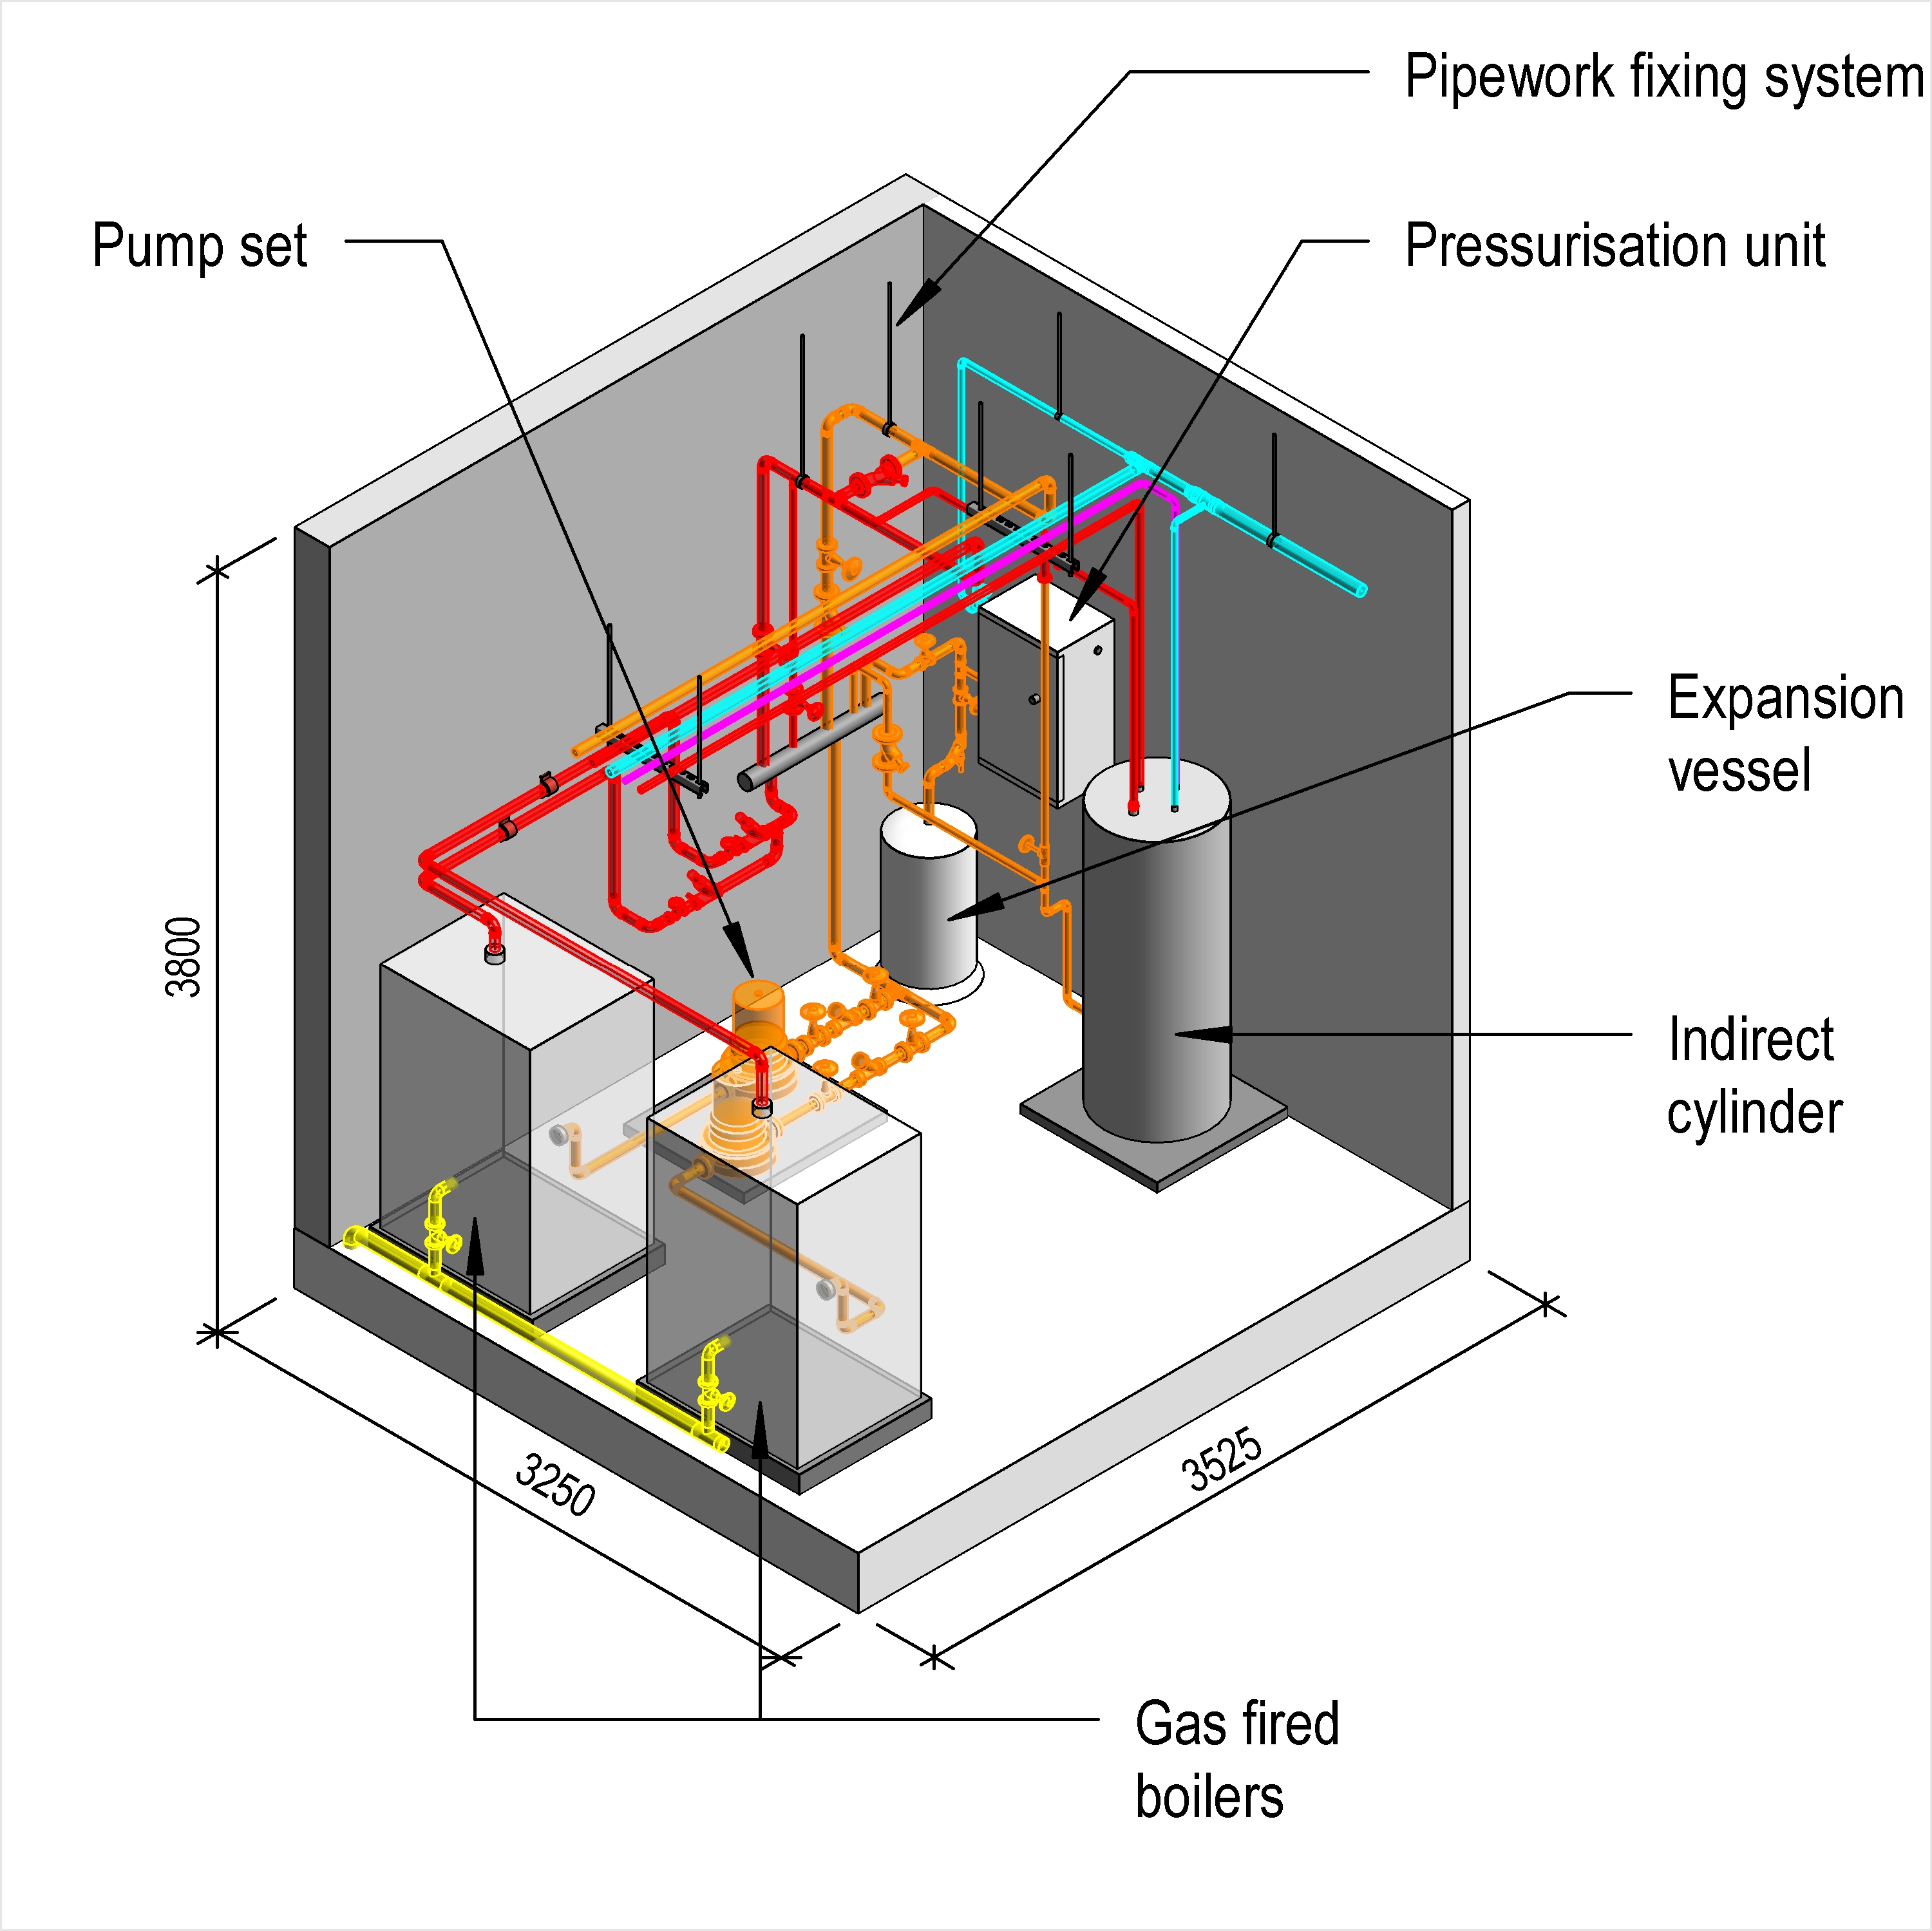
\includegraphics[width=\textwidth]{figures/MTHW-heating-systems.jpg}
		\rule{\textwidth}{0.5pt} % use line???
  \caption{NBS LoD 5}
  \label{}
\end{subfigure}
  \begin{subfigure}[b]{.61\textwidth}
  \centering
  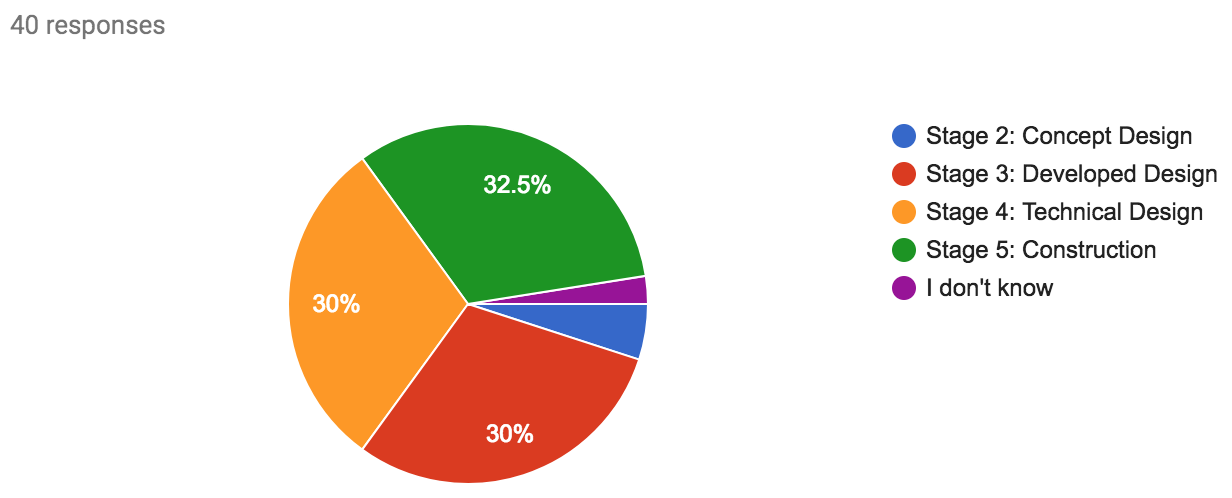
\includegraphics[width=\textwidth]{figures/image1.png}
 		\rule{\textwidth}{0.5pt} % use line???
  \caption{Responses}
  \label{}
\end{subfigure}
\caption[The actual and guessed LoDs of the first image in the ``Match the Image with the Work Stage" activity.]{({\scriptsize A}) The actual LoD and ({\scriptsize B}) the respondents’ guessed LoD of the first image in the ``Match the Image with the Work Stage" activity.}
\label{image1}
\end{figure}
%%%



%%% 2
\begin{figure}[htbp]
\centering
  \begin{subfigure}[b]{.35\textwidth}
  \centering
  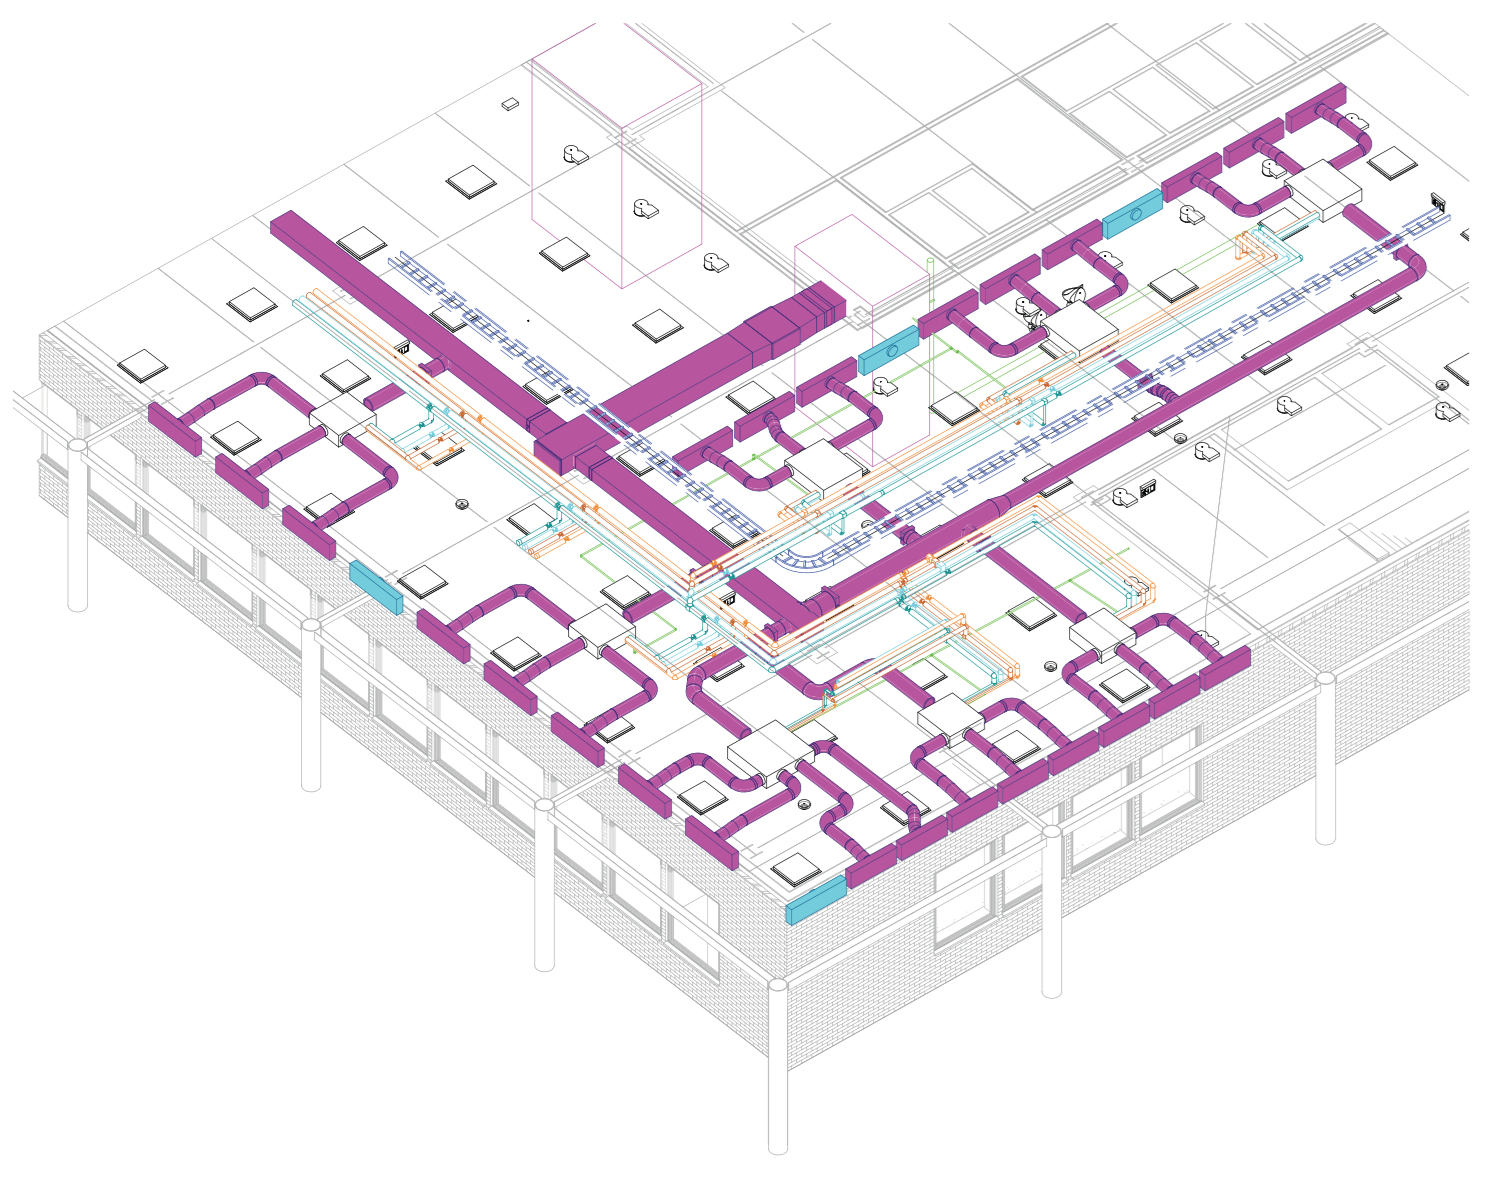
\includegraphics[width=\textwidth]{figures/4bModel01.png}
 		\rule{\textwidth}{0.5pt} % use line???
  \caption{BG6 Model Definition 4b}
  \label{}
\end{subfigure}
  \begin{subfigure}[b]{.61\textwidth}
  \centering
  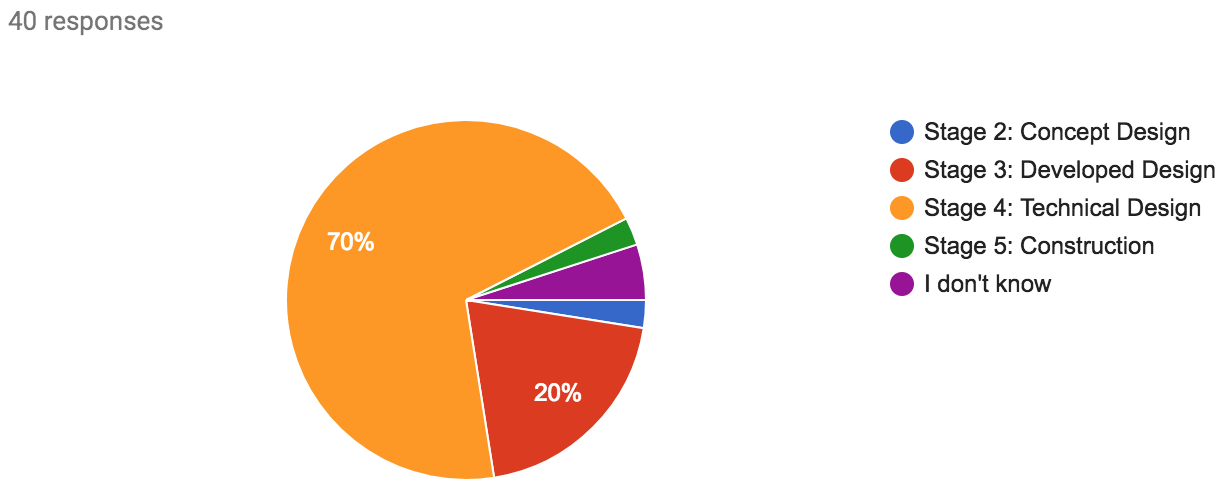
\includegraphics[width=\textwidth]{figures/image2.png}
		\rule{\textwidth}{0.5pt} % use line???
  \caption{Responses}
  \label{}
\end{subfigure}
\caption[The actual and guessed LoDs of the second image in the ``Match the Image with the Work Stage" activity.]{({\scriptsize A}) The actual LoD and ({\scriptsize B}) the respondents’ guessed LoD of the second image in the ``Match the Image with the Work Stage" activity.}
\label{image2}
\end{figure}
%%%



%%% 3
\begin{figure}[htbp]
\centering
  \begin{subfigure}[b]{.35\textwidth}
  \centering
  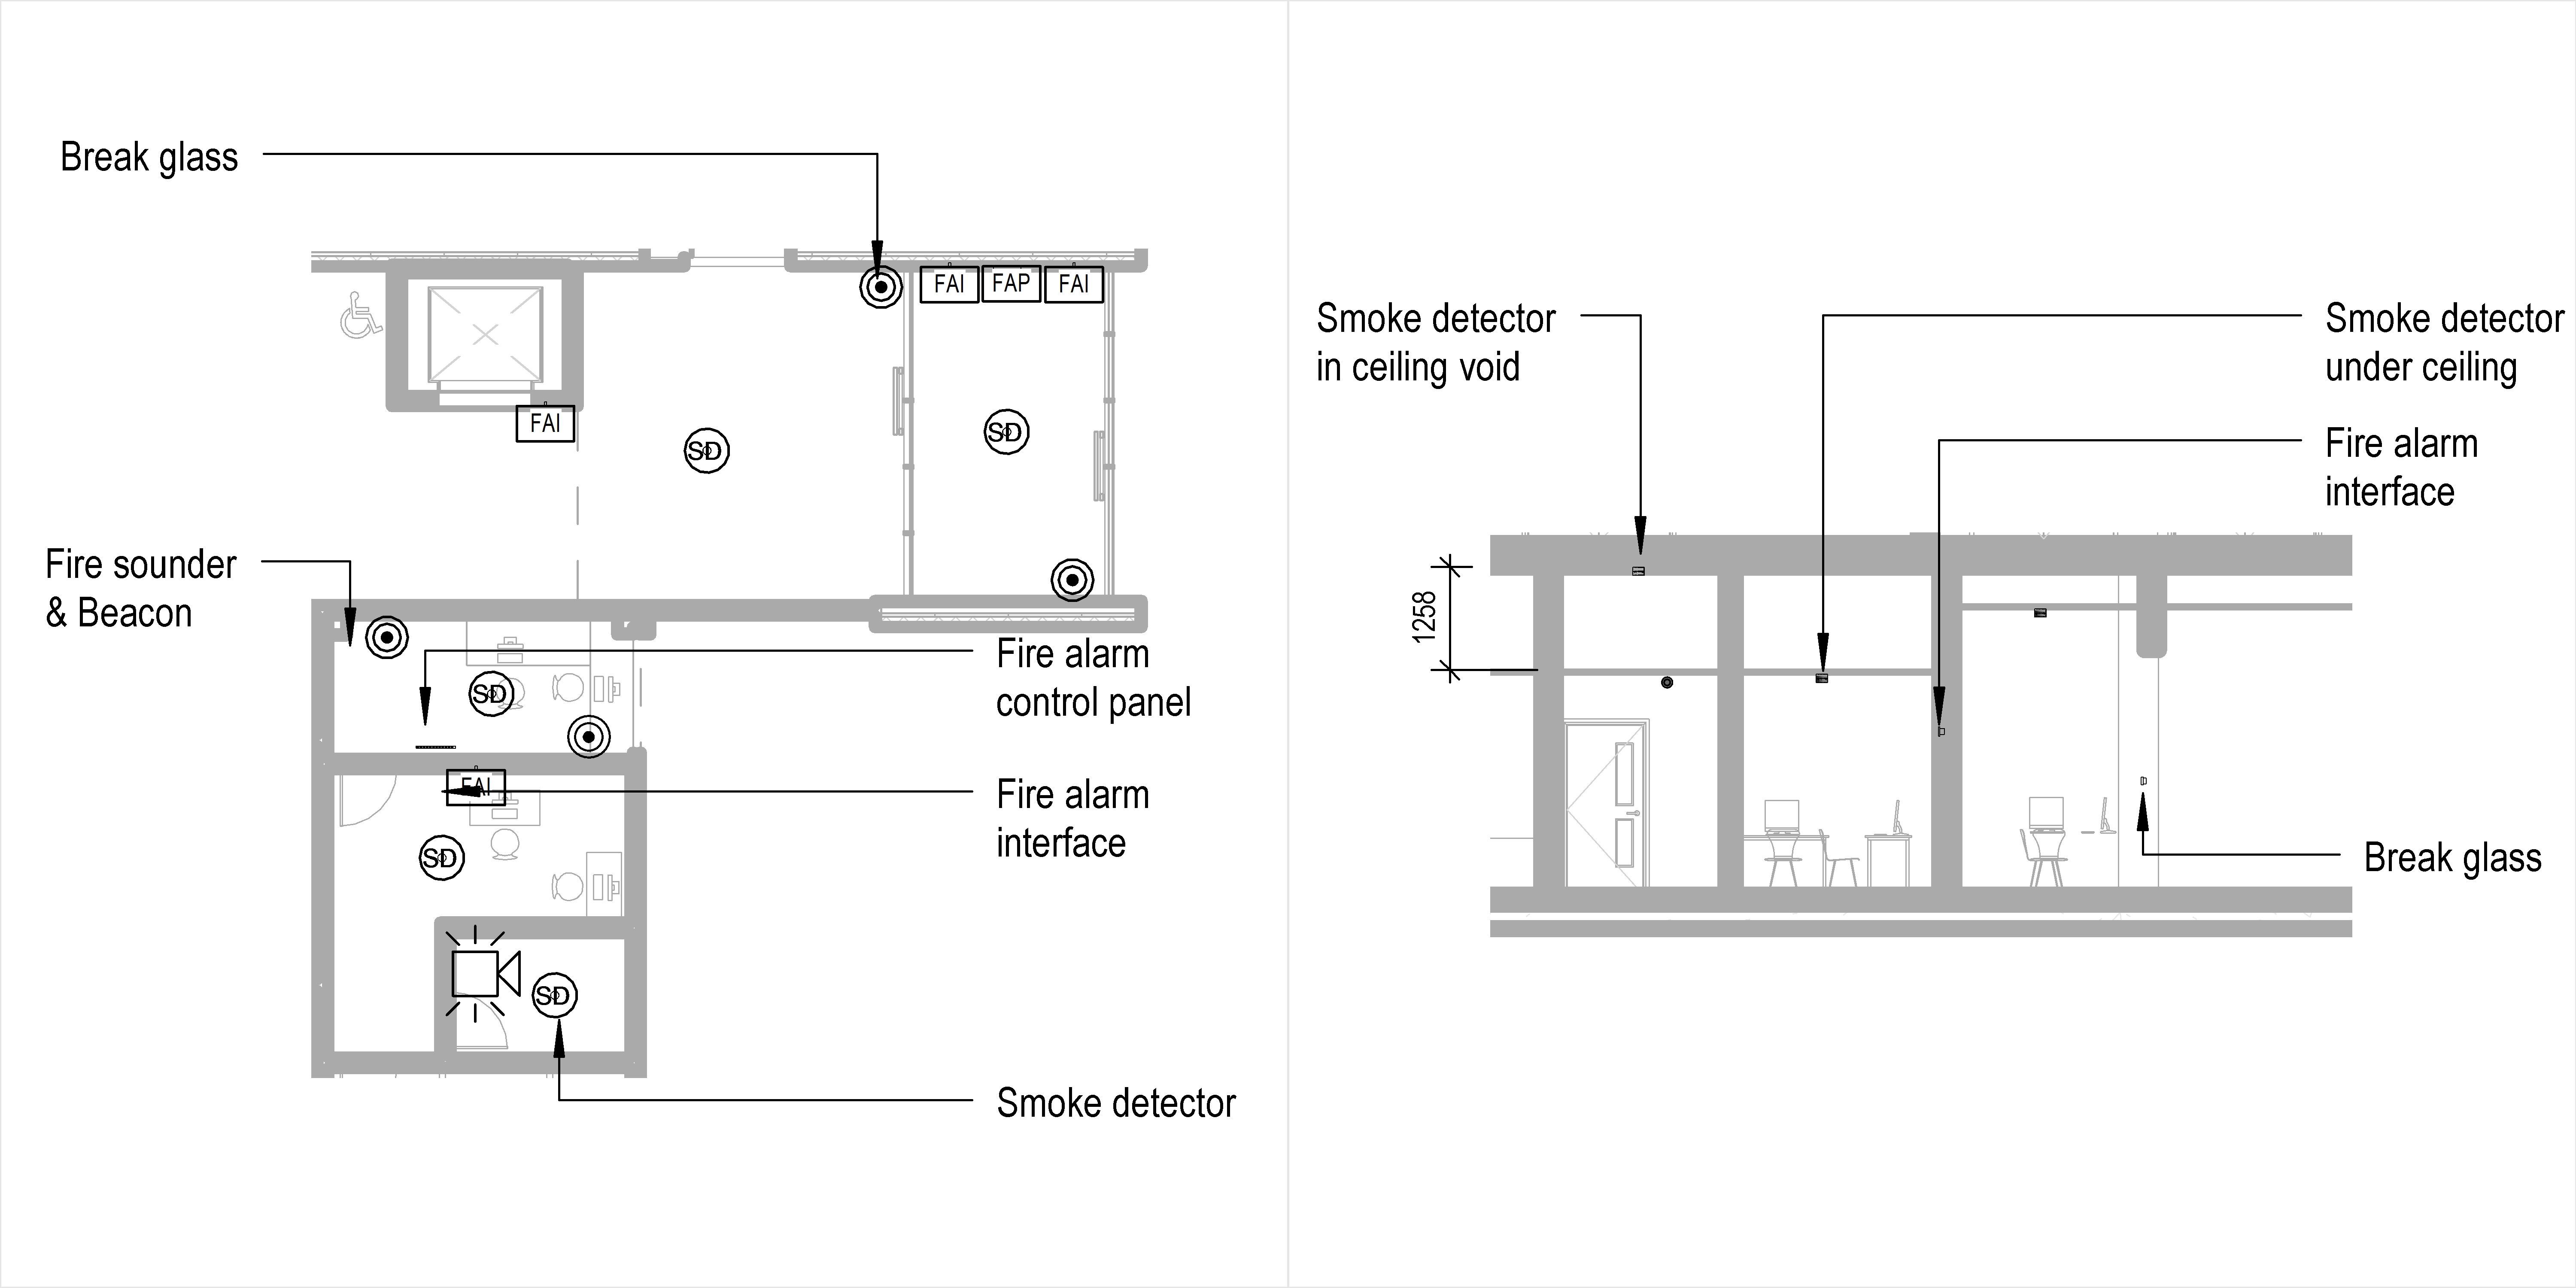
\includegraphics[width=\textwidth]{figures/fire-combined.png}
		\rule{\textwidth}{0.5pt} % use line???
  \caption{NBS LoD 4}
  \label{}
\end{subfigure}
  \begin{subfigure}[b]{.61\textwidth}
  \centering
  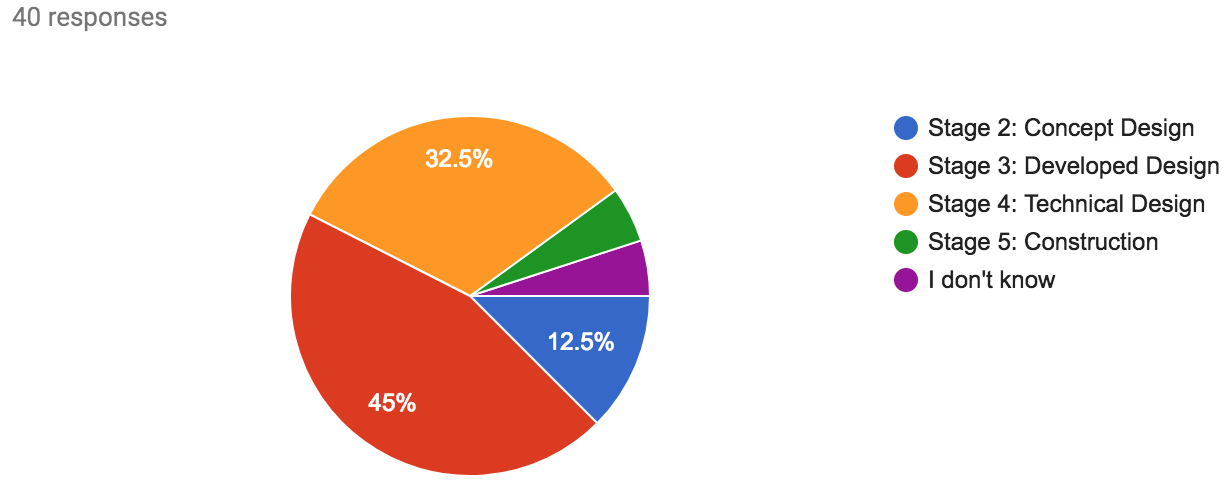
\includegraphics[width=\textwidth]{figures/image3.png}
		\rule{\textwidth}{0.5pt} % use line???
  \caption{Responses}
  \label{}
\end{subfigure}
\caption[The actual and guessed LoDs of the third image in the ``Match the Image with the Work Stage" activity.]{({\scriptsize A}) The actual LoD and ({\scriptsize B}) the respondents’ guessed LoD of the third image in the ``Match the Image with the Work Stage" activity.}
\label{image3}
\end{figure}
%%%



%%% 4
\begin{figure}[htbp]
\centering
  \begin{subfigure}[b]{.35\textwidth}
  \centering
  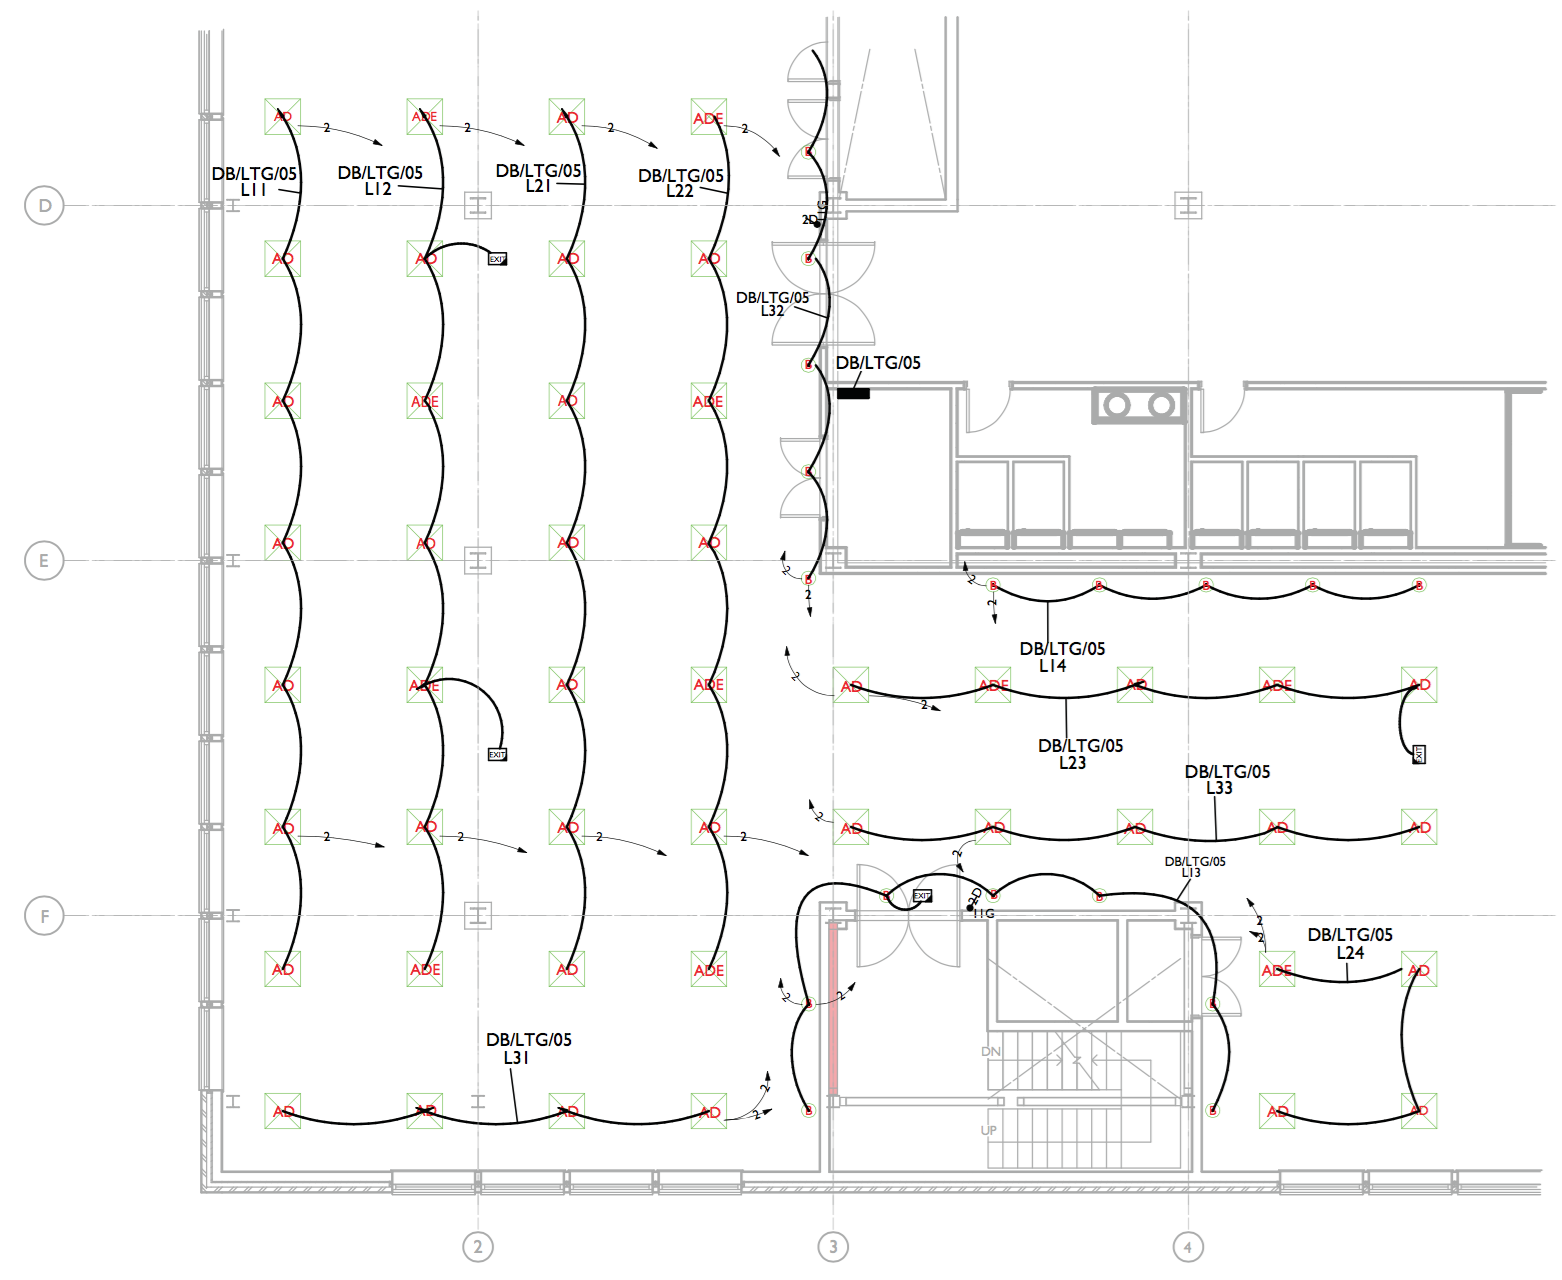
\includegraphics[width=\textwidth]{figures/4aDwg02.png}
		\rule{\textwidth}{0.5pt} % use line???
  \caption{BG6 Drawing Definition 4a}
  \label{}
\end{subfigure}
  \begin{subfigure}[b]{.61\textwidth}
  \centering
  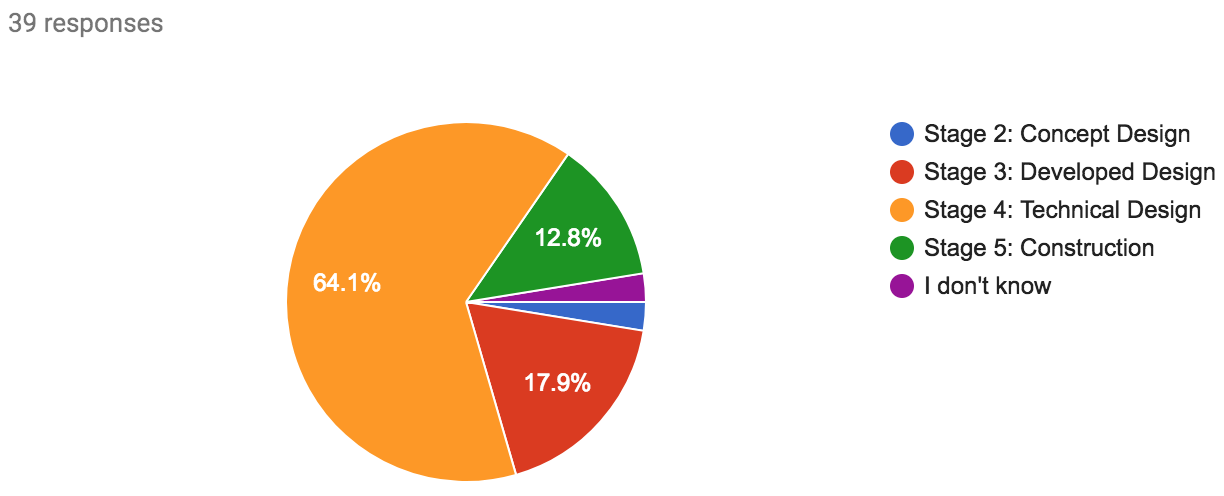
\includegraphics[width=\textwidth]{figures/image4.png}
		\rule{\textwidth}{0.5pt} % use line???
  \caption{Responses}
  \label{}
\end{subfigure}
\caption[The actual and guessed LoDs of the fourth image in the ``Match the Image with the Work Stage" activity.]{({\scriptsize A}) The actual LoD and ({\scriptsize B}) the respondents’ guessed LoD of the fourth image in the ``Match the Image with the Work Stage" activity.}
\label{image4}
\end{figure}
%%%



%%% 5
\begin{figure}[htbp]
\centering
  \begin{subfigure}[b]{.35\textwidth}
  \centering
  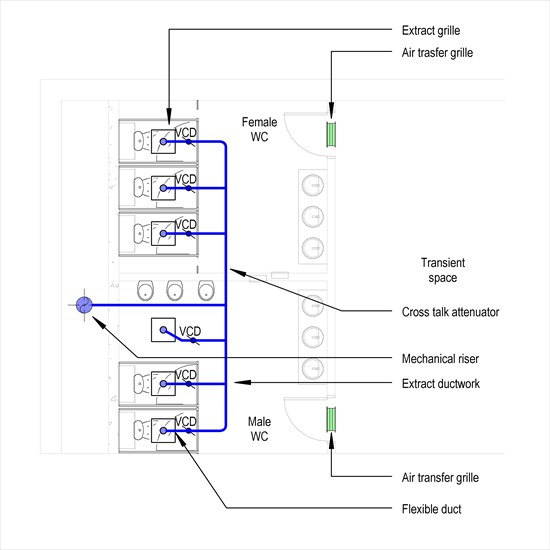
\includegraphics[width=\textwidth]{figures/local-exhaust-vent-syst.jpg}
		\rule{\textwidth}{0.5pt} % use line???
  \caption{NBS LoD 3}
  \label{}
\end{subfigure}
  \begin{subfigure}[b]{.61\textwidth}
  \centering
  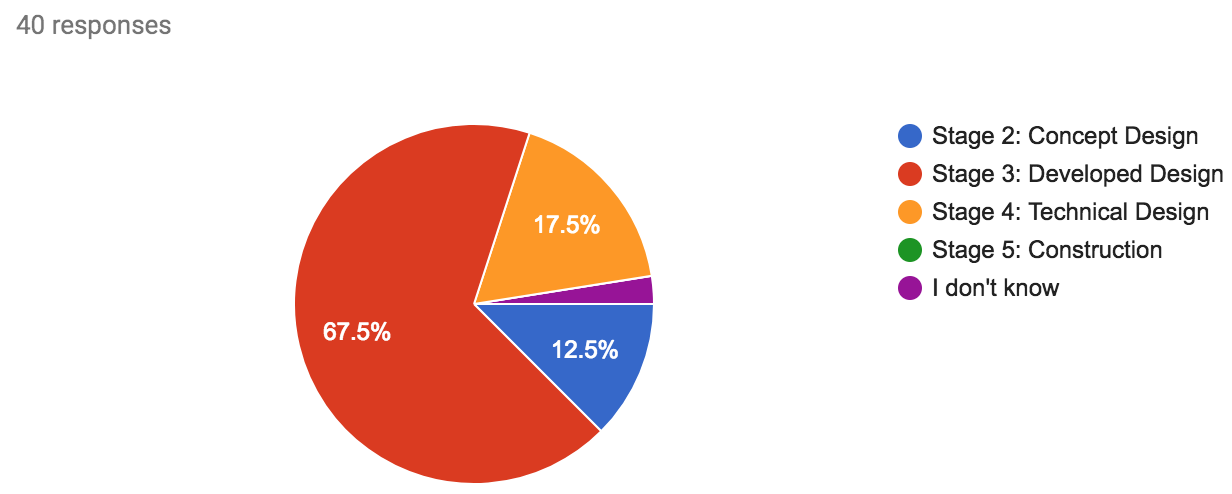
\includegraphics[width=\textwidth]{figures/image5.png}
		\rule{\textwidth}{0.5pt} % use line???
  \caption{Responses}
  \label{}
\end{subfigure}
\caption[The actual and guessed LoDs of the fifth image in the ``Match the Image with the Work Stage" activity.]{({\scriptsize A}) The actual LoD and ({\scriptsize B}) the respondents’ guessed LoD of the fifth image in the ``Match the Image with the Work Stage" activity.}
\label{image5}
\end{figure}
%%%



%%% 6
\begin{figure}[htbp]
\centering
  \begin{subfigure}[b]{.35\textwidth}
  \centering
  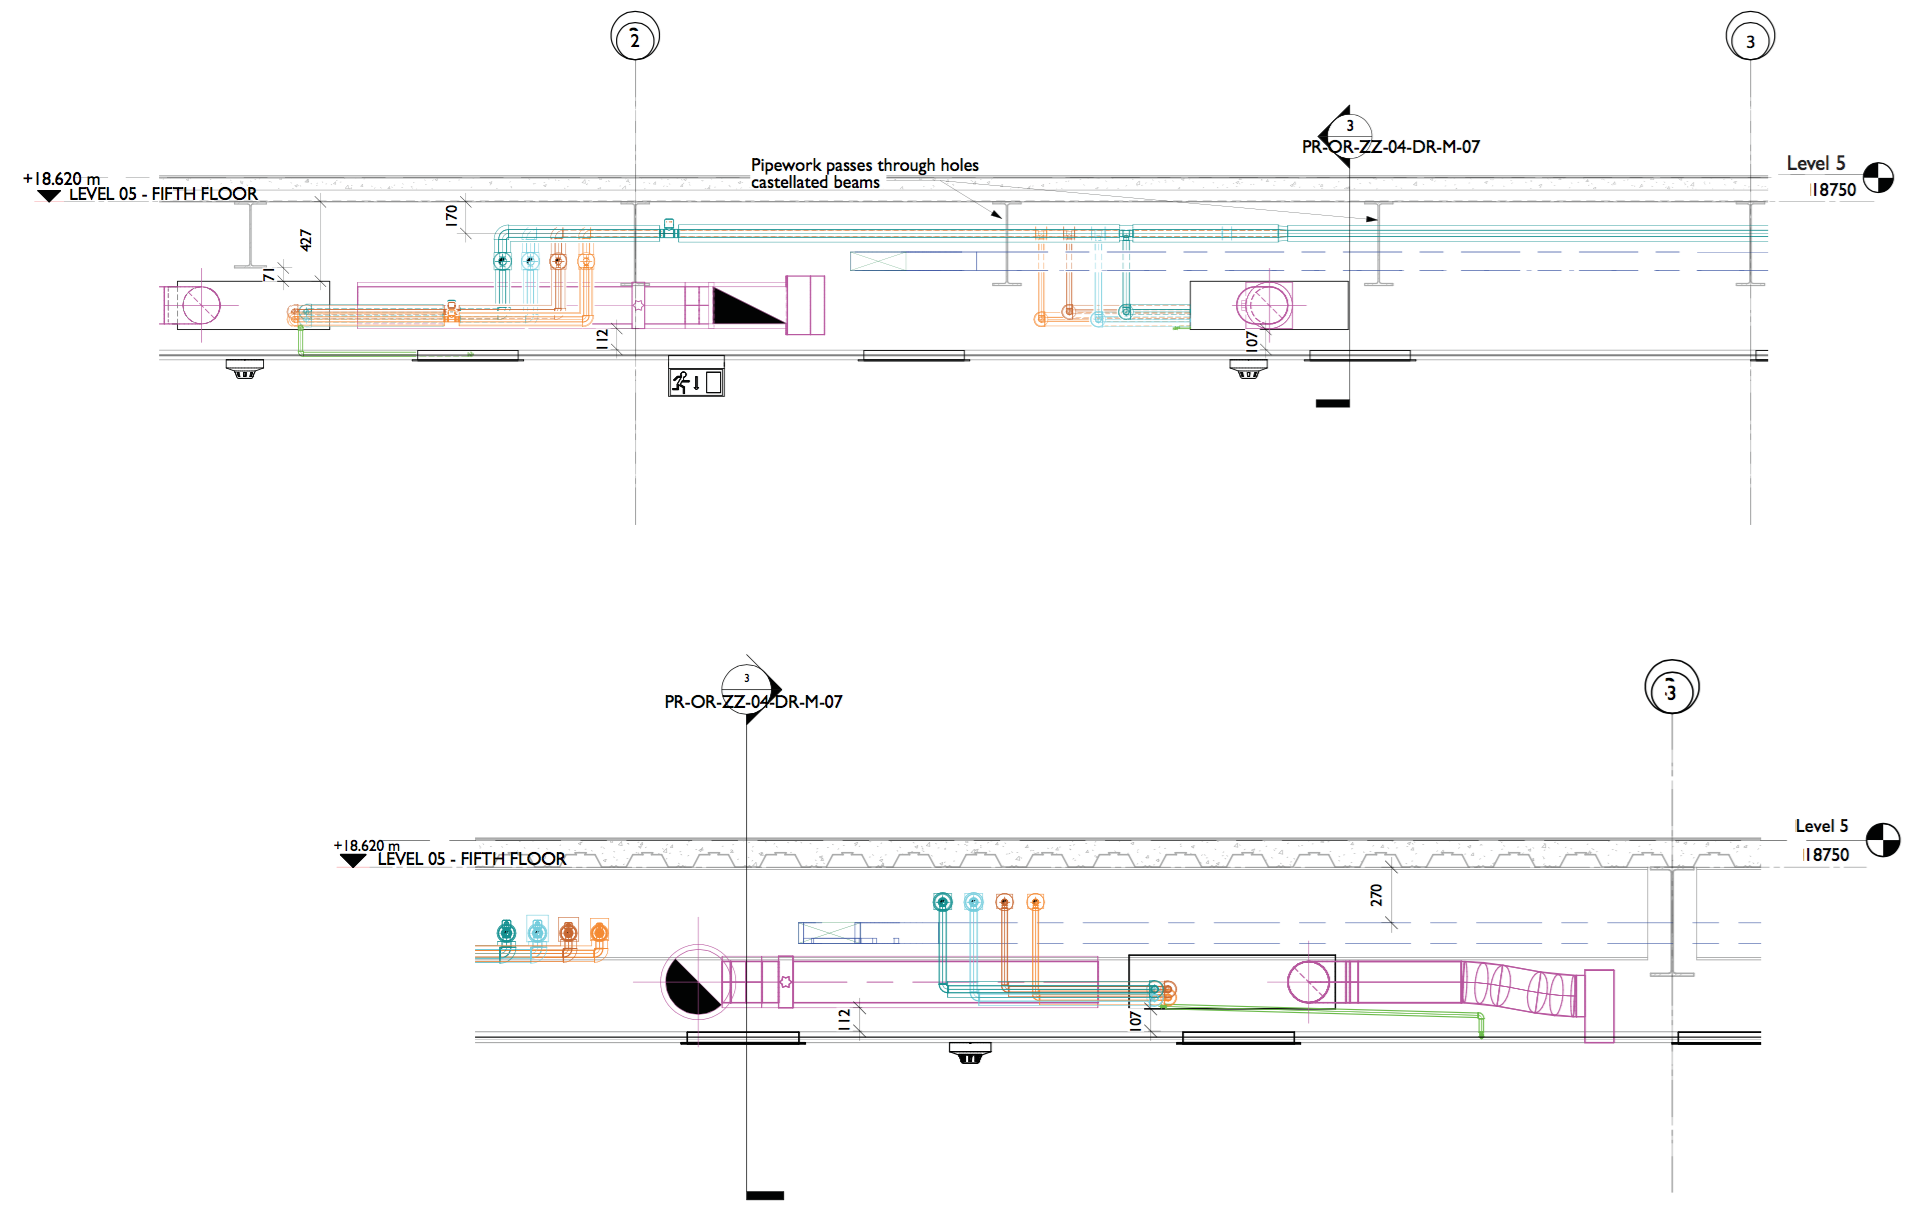
\includegraphics[width=\textwidth]{figures/4bCoordDwg02.png}
		\rule{\textwidth}{0.5pt} % use line???
  \caption{BG6 Drawing Definition 4b}
  \label{}
\end{subfigure}
  \begin{subfigure}[b]{.61\textwidth}
  \centering
  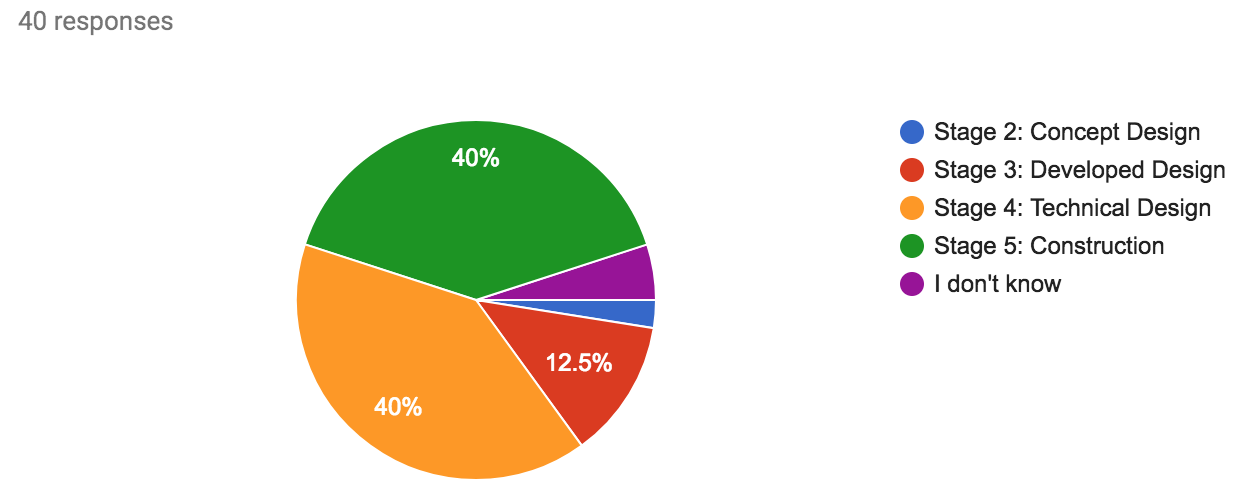
\includegraphics[width=\textwidth]{figures/image6.png}
		\rule{\textwidth}{0.5pt} % use line???
  \caption{Responses}
  \label{}
\end{subfigure}
\caption[The actual and guessed LoDs of the sixth image in the ``Match the Image with the Work Stage" activity.]{({\scriptsize A}) The actual LoD and ({\scriptsize B}) the respondents’ guessed LoD of the sixth image in the ``Match the Image with the Work Stage" activity.}
\label{image6}
\end{figure}
%%%




%------------------------------
%	SUBSECTION 6
%------------------------------

\newpage
\subsection{Documents}

This section of the questionnaire asked the respondents if they were familiar with PAS 1192-2, BG 6 and ACE Schedule of Services MEP (see Figures \ref{pas} to \ref{ace}).
The respondents were most familiar with the BG 6, and least familiar with the ACE Schedule of Services MEP.

% PIE CHART
\begin{figure}[htbp]
	\centering
	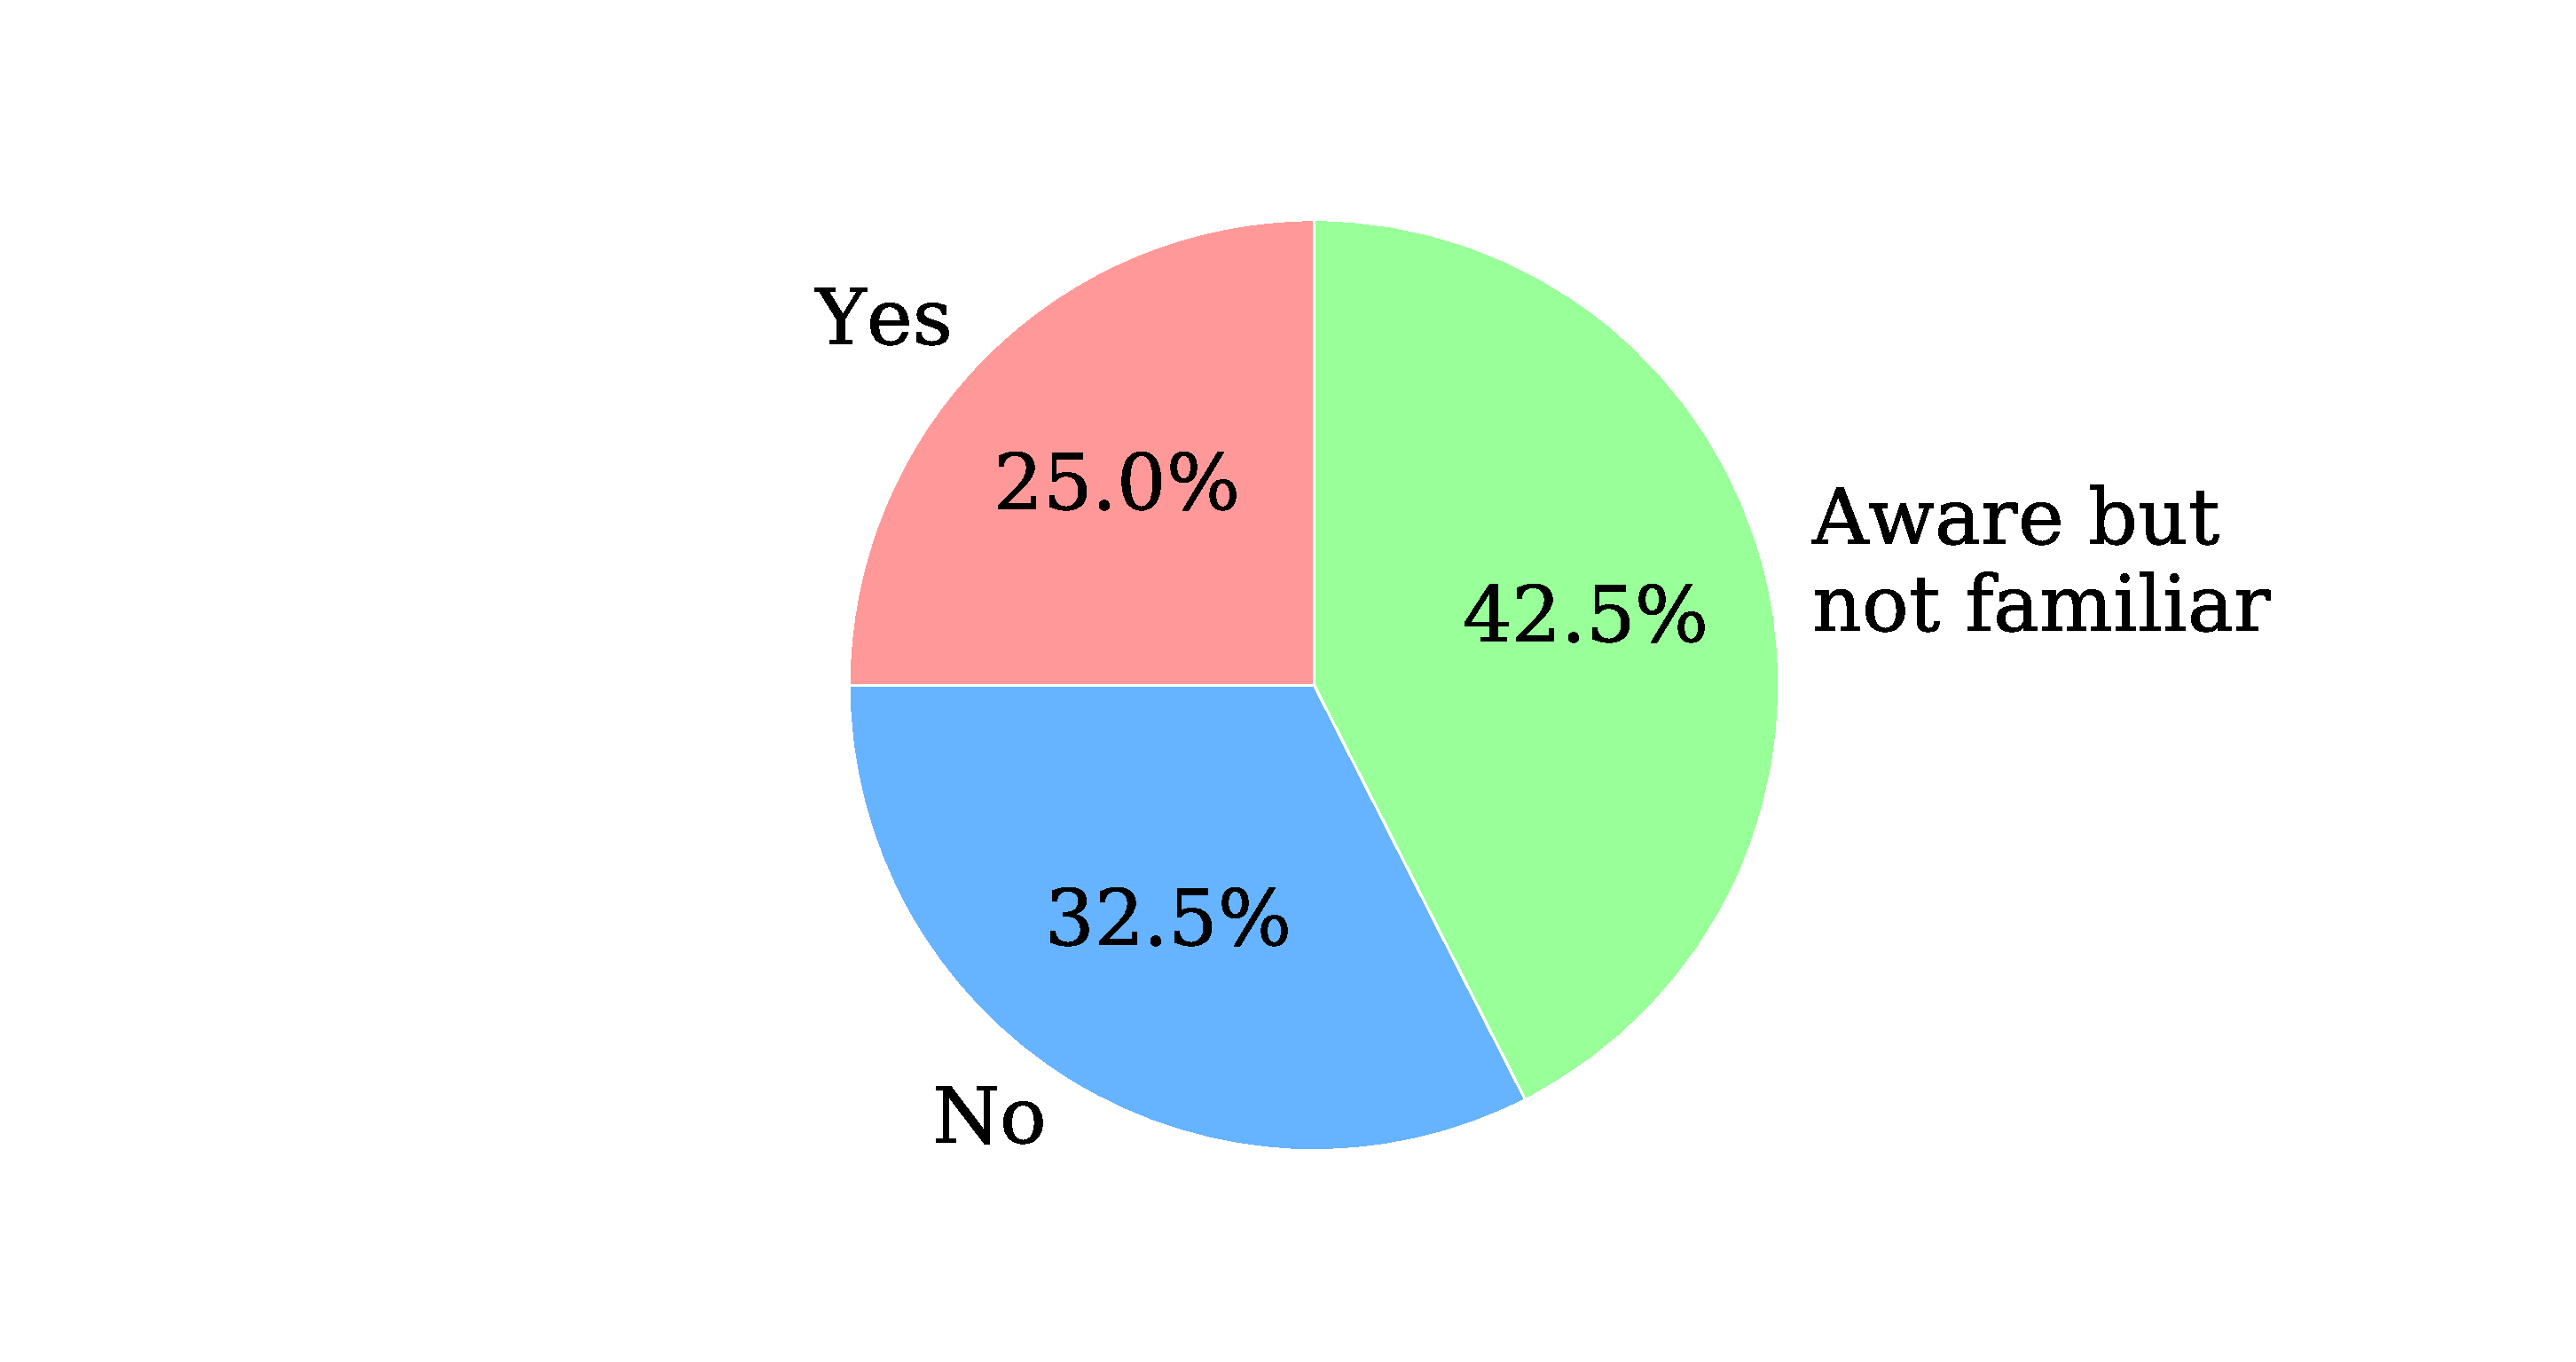
\includegraphics[width=0.6\textwidth]{figures/PAS_1192-2.eps}
	\rule{0.8\textwidth}{0.5pt} % use line???
	\caption{Respondents' familiarity with PAS 1192-2.}
	\label{pas}
\end{figure}


% PIE CHART
\begin{figure}[htbp]
	\centering
	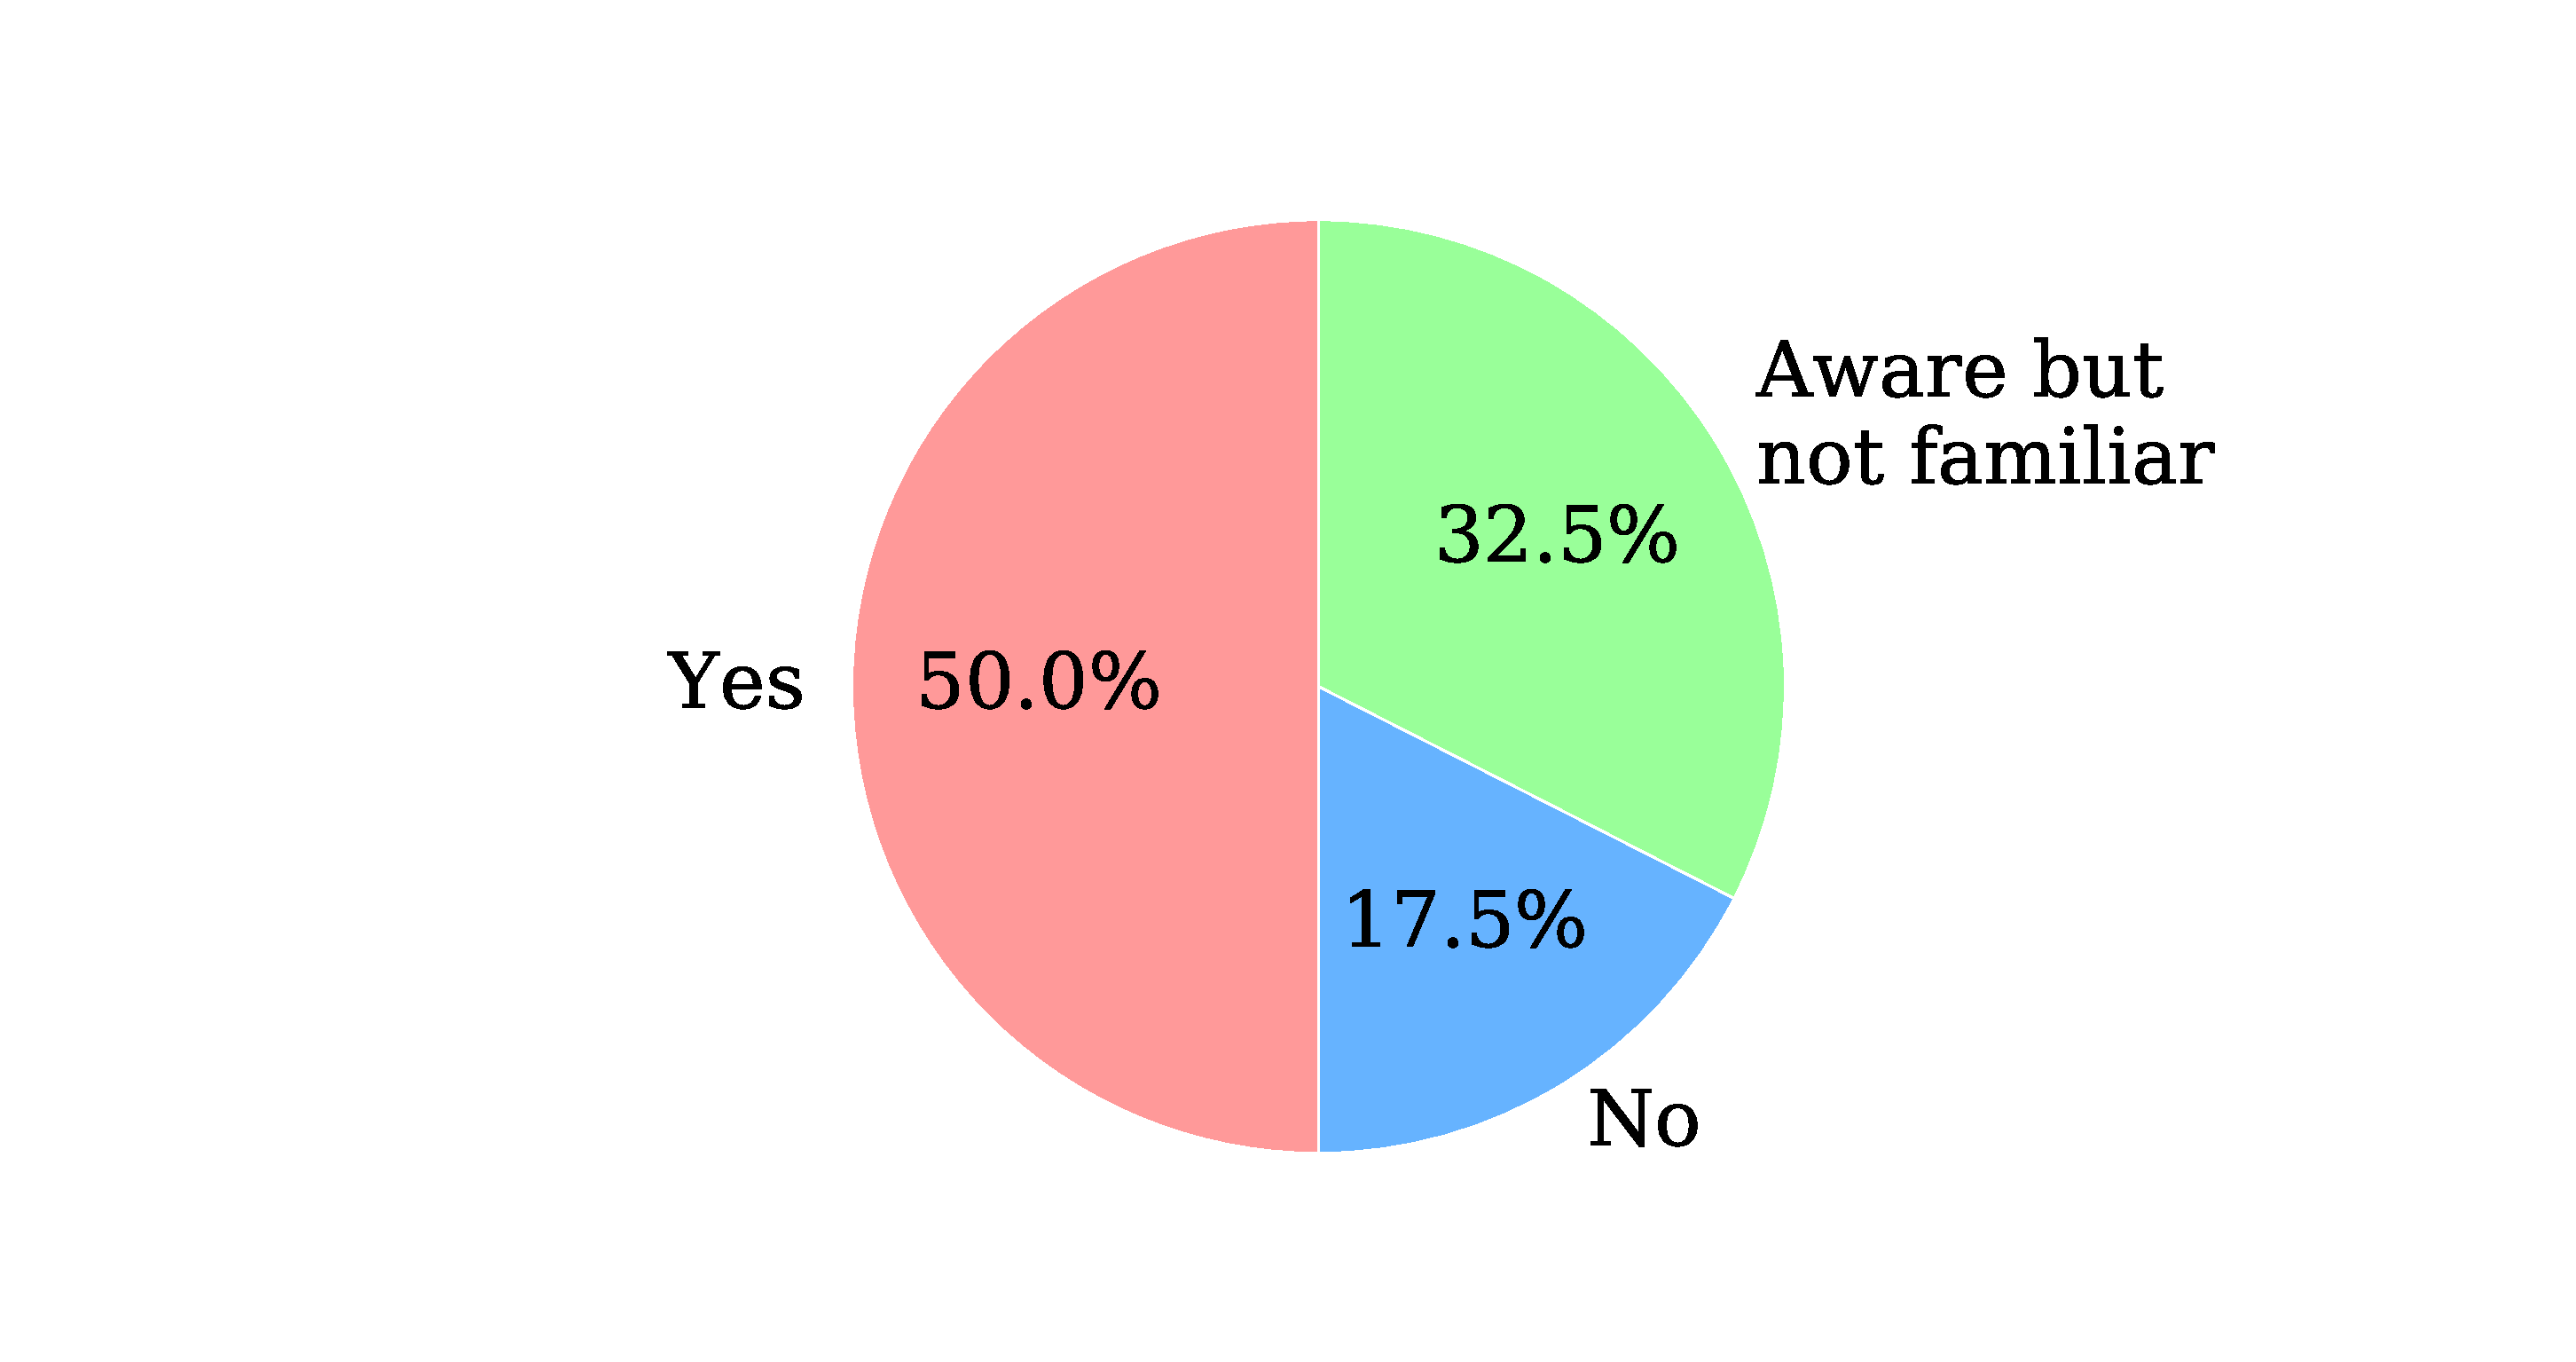
\includegraphics[width=0.6\textwidth]{figures/BG6.eps}
	\rule{0.8\textwidth}{0.5pt} % use line???
	\caption{Respondents' familiarity with BG 6.}
	\label{bg6}
\end{figure}


% PIE CHART
\begin{figure}[htbp]
	\centering
	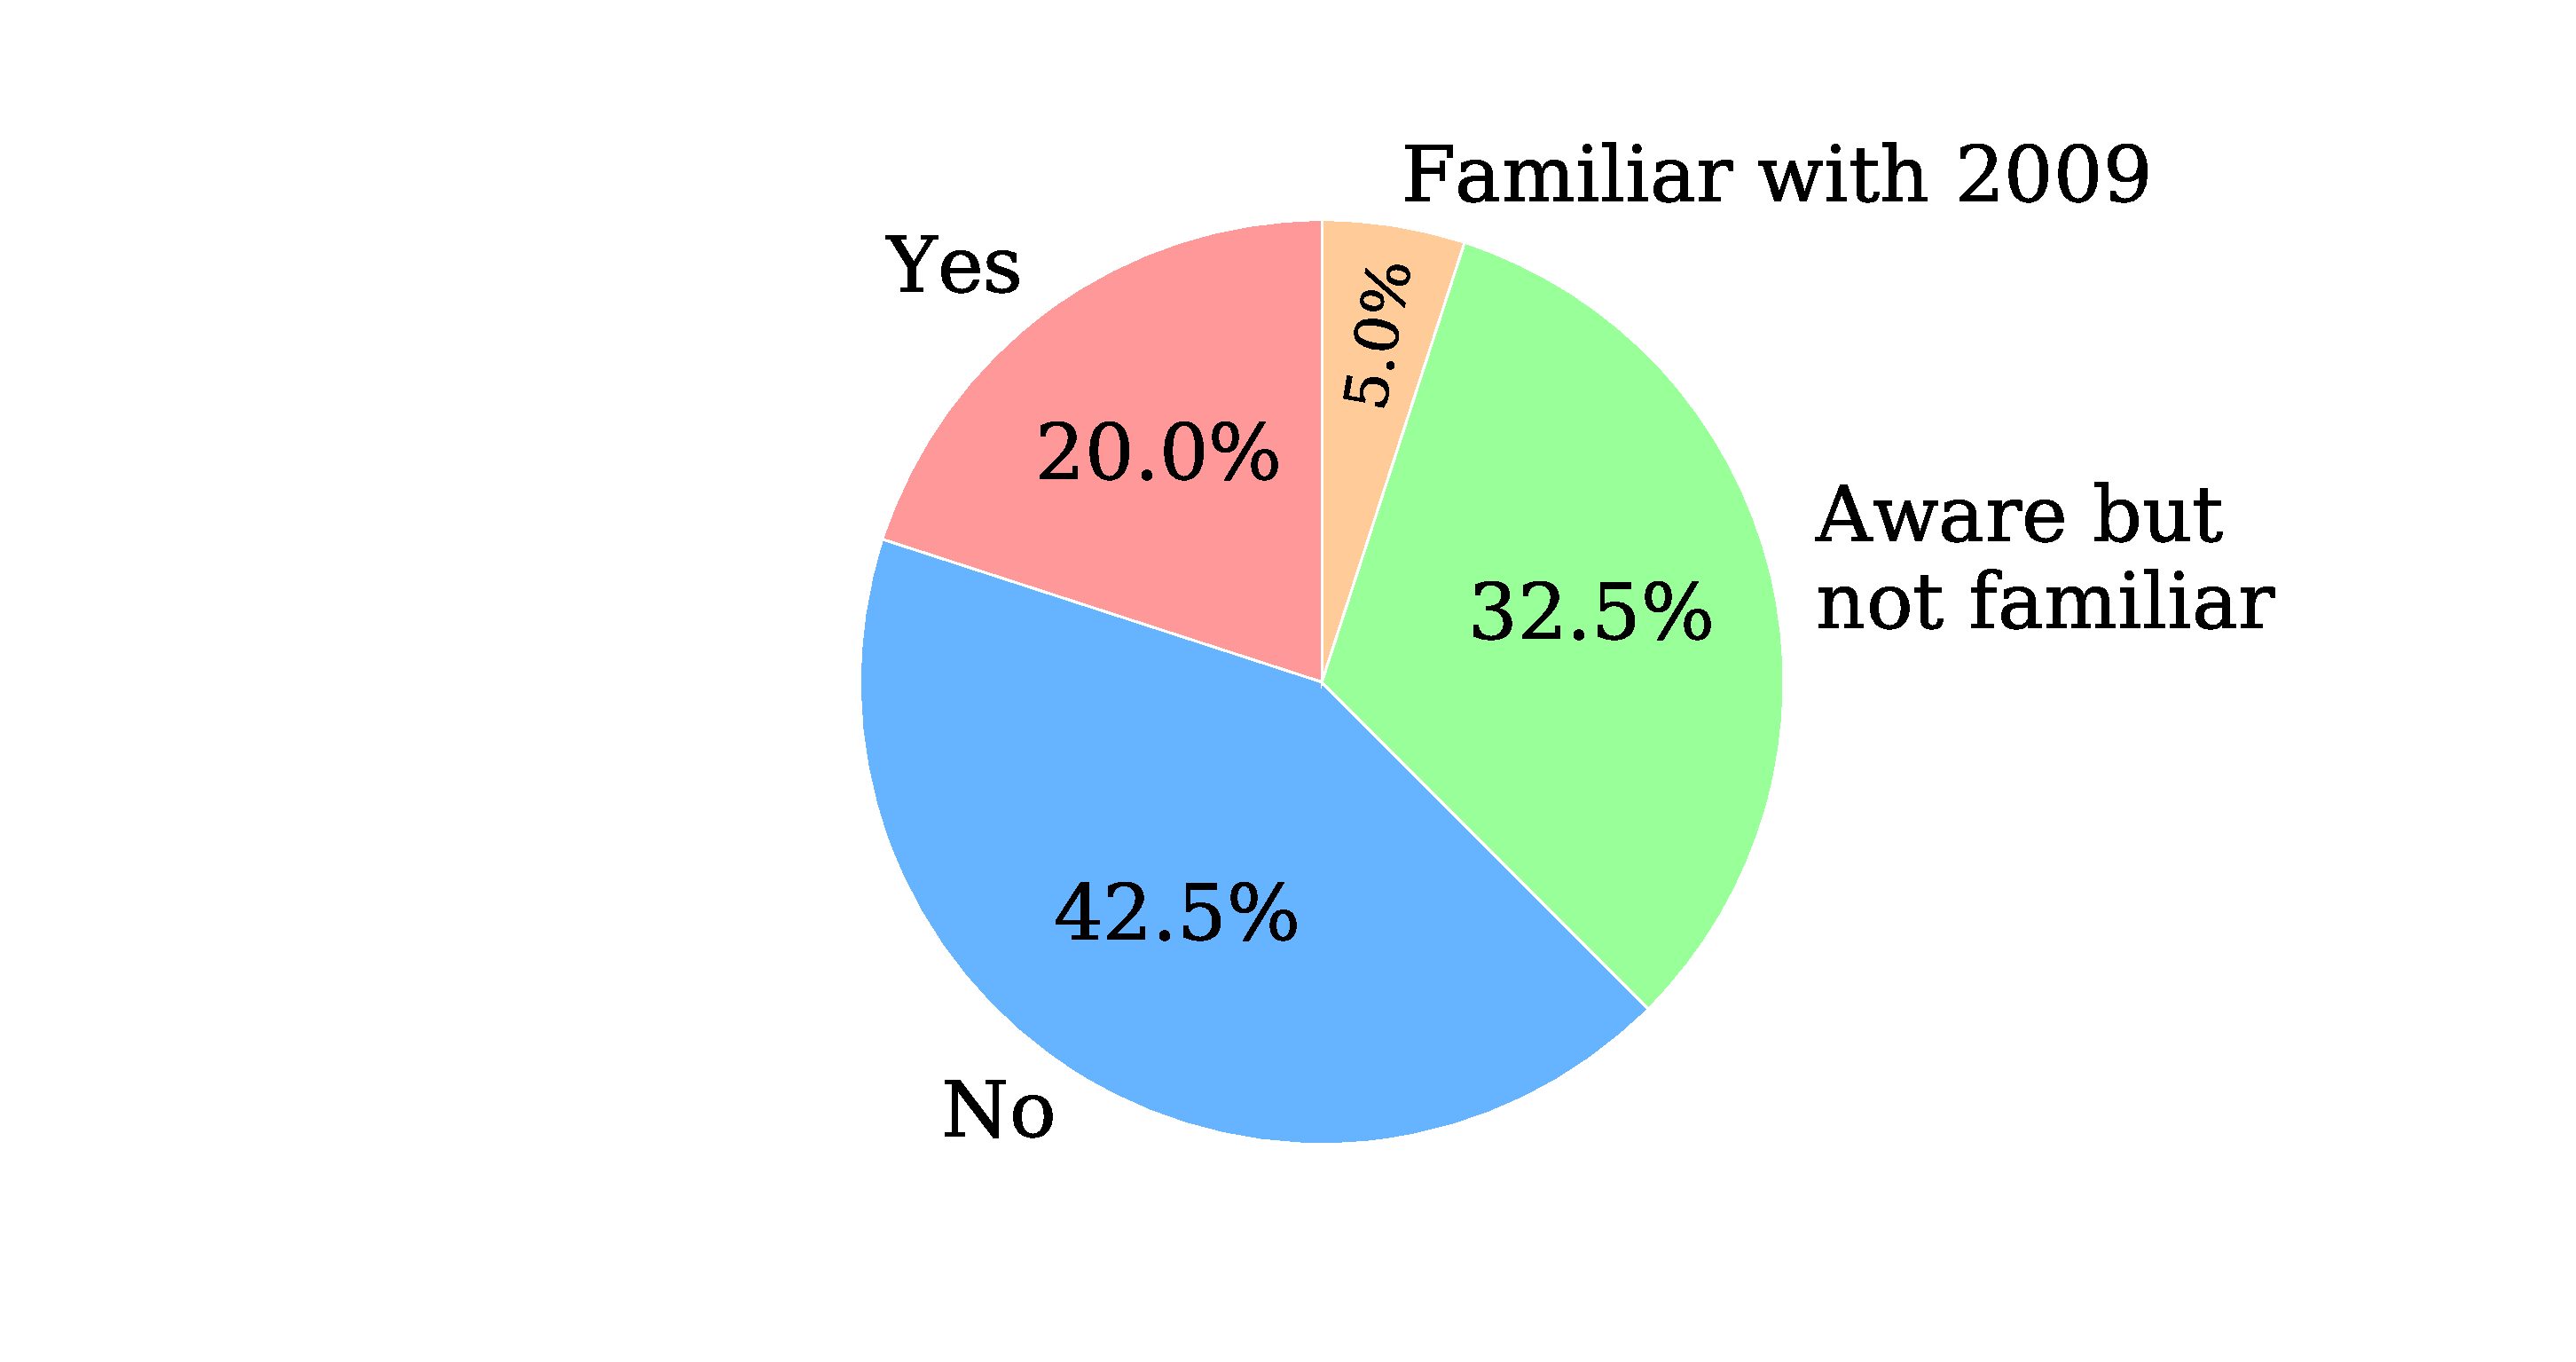
\includegraphics[width=0.6\textwidth]{figures/ACE.eps}
	\rule{0.8\textwidth}{0.5pt} % use line???
	\caption{Respondents' familiarity with ACE Schedule of Services \\ MEP 2017 Edition.}
	\label{ace}
\end{figure}

%% PAS
% 67.5\% of the respondents were aware or familiar with PAS 1192-2.
Figure \ref{BIM_literacy_X_PAS1192} shows the respondents' familiarity with PAS 1192-2 in terms of their BIM literacy.
Since PAS 1192-2 is the industry standard for BIM process during the CAPEX phase of a project, it is interesting to note that 20\% of the respondents agreed to being BIM literate without being familiar with or even aware of the document.
% , yet they have either never heard of or are not familiar with the PAS 1192-2:2013.

% BAR CHART
\begin{figure}[htbp]
	\centering
	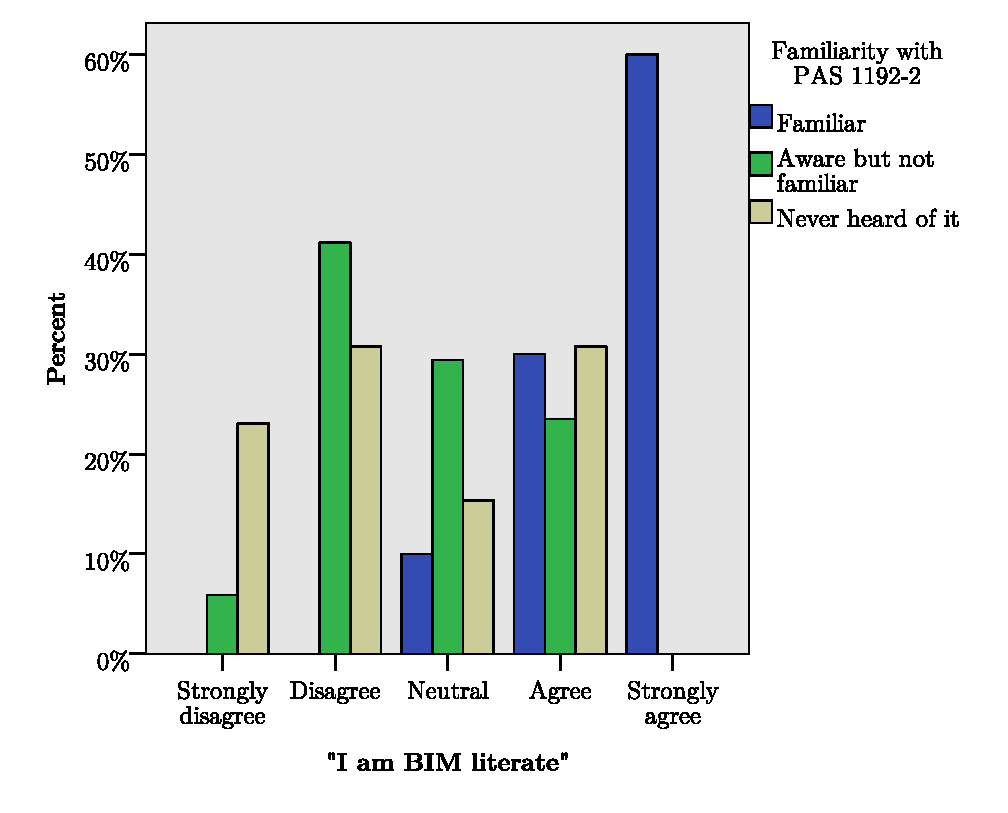
\includegraphics[width=0.9\textwidth]{figures/BimLiteracyXPas1192Percent.eps}
	\rule{0.9\textwidth}{0.5pt} % use line???
	\caption{Respondents' familiarity with PAS 1192-2:2013 in terms of their BIM literacy}
	\label{BIM_literacy_X_PAS1192}
\end{figure}



%% BG6
From Figure \ref{BG6_X_BS_fields} it can be observed that all respondents that have worked in MEP services are aware of or familiar with the BG 6.
% 65.5\% of the MEP respondents are familiar with the document.
Those who have never heard of the BG 6 are composed of specialist building services engineers and people who have not worked in building services.

% BAR CHART
\begin{figure}[htbp]
	\centering
	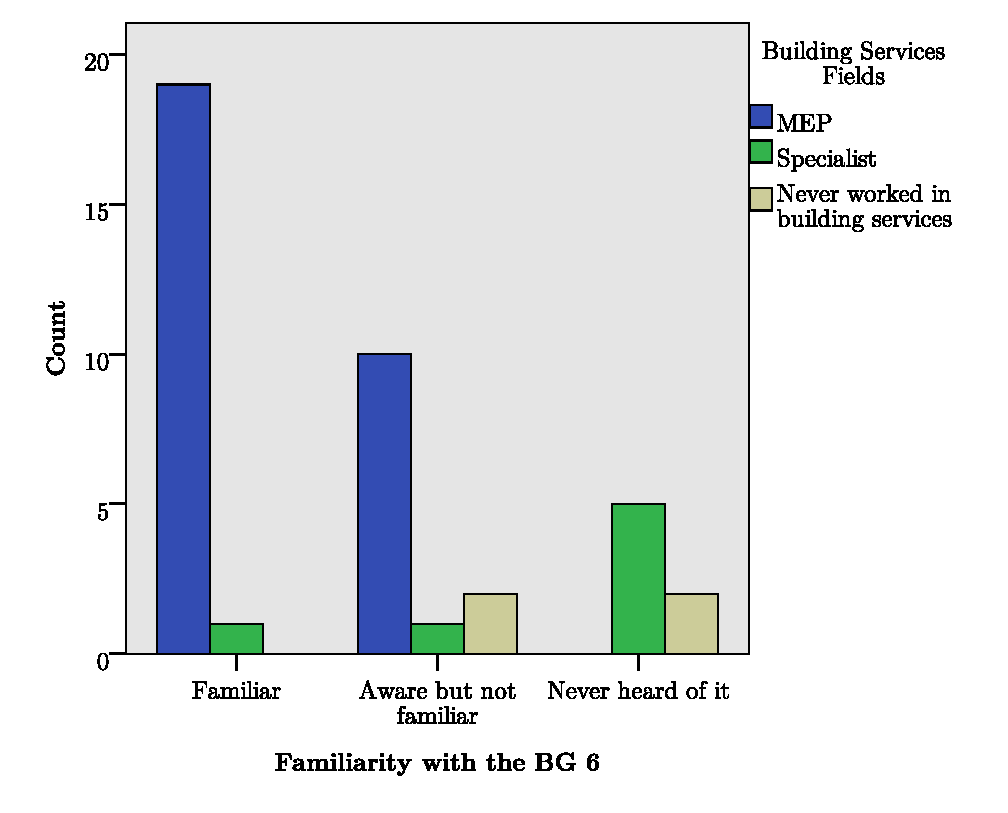
\includegraphics[width=0.9\textwidth]{figures/Bg6XBsFieldsCount.eps}
	\rule{0.9\textwidth}{0.5pt} % use line???
	\caption{Respondents' familiarity with BG6 in terms of building services fields}
	\label{BG6_X_BS_fields}
\end{figure}



%% ACE
Only 25\% of the respondents are familiar with either the 2009 or 2017 (current) edition of the ACE Schedule of Services MEP (see Figure \ref{ace}).
These respondents are either MEP or specialist building services engineers (see Figure \ref{ACE_X_BS_fields}).
As the ACE Schedule of Services MEP is aimed at MEP engineers, it is interesting to note that 72.4\% of the MEP respondents are not familiar with either of the ACE documents.

% BAR CHART
\begin{figure}[htbp]
	\centering
	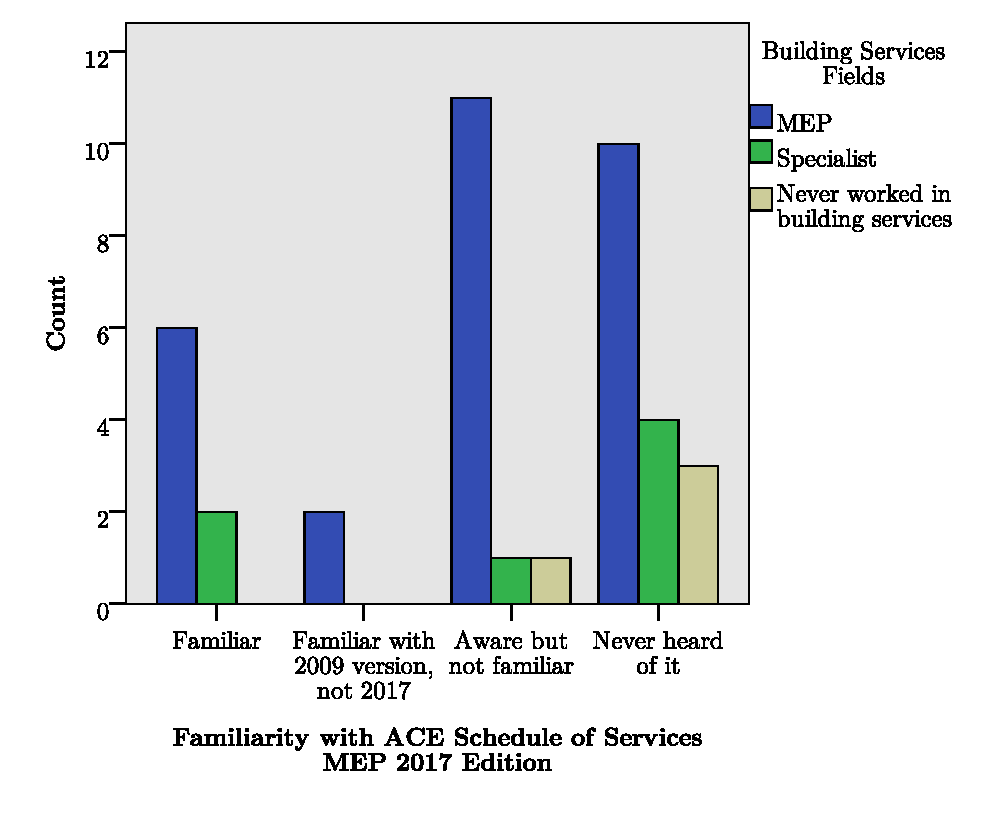
\includegraphics[width=0.9\textwidth]{figures/AceXBsFieldsCount.eps}
	\rule{0.9\textwidth}{0.5pt} % use line???
	\caption{Respondents' familiarity with ACE document in terms of building services fields}
	\label{ACE_X_BS_fields}
\end{figure}








%----------------------------------------------------------------------------------------
%	SECTION 2
%----------------------------------------------------------------------------------------

\section{Follow-Up Interviews}

Four of the survey respondents were approached to participate in follow-up interviews, and two agreed to this.
Both interviewees were experienced MEP contractors: the first worked for a subsidiary of a multinational construction company with over 15,000 employees, and the second worked for a smaller UK construction and engineering company.
The questions used in the interviews can be found in Appendices \ref{AppendixB} and \ref{AppendixC}.

\begin{comment}
\hl{
So far I have identified three people that I would like to have a follow-up interview with: two contractors and one BIM manager/ coordinator.
Should I also speak with a consulting engineer and a policy/ regulation consultant?
If so, perhaps Jon (mechanical engineer, former placement supervisor, plus descriptive in LOD question) and Stefan (consultant)?
(Don't want to have too many interviews to process either...)
}
\end{comment}


%------------------------------
%	SUBSECTION 1
%------------------------------

\subsection{First Interview}

\begin{comment}
\hl{Introduce him...}

MEP contractor.
Work exclusively for LoR.
In other circumstances, would be classed as Tier 2 contractor (sub-contractor to a main contractor).
Primary activity: installation, commissioning and handover of building services on a construction project.
\end{comment}

The first interviewee is the head of information management (a.k.a. BIM management) at their company.
Their team's primary responsibility is the production of information, models and drawings for the installation of MEP services and off-site manufacture.
% Their team produces all the models and drawings for installation and off-site manufacture.
They typically receive information from consultants at Stage 4a (but sometimes also at Stage 3) and develop it to Stage 5.
% at stage 3 or early stage 4, develop it to stage 5.
% More often than not, involved from stage 4a.
However, the interviewee explains that, to make for a practical consultant-to-contractor handover, they would seek to be appointed at Stage 3.
\say{Where we have the opportunity to engage early with our client and the design consultant, for example at Stage 3, then we will be able to influence and guide the development of the model and the design through to Stage 4a. And in those instances we'll get a model that is more useful to us.
Where we enter onto a project where we haven't been engaged early, and we receive a model at Stage 4a, then, more often than not, we need to do a lot of re-work. 
So our strategy is that, where possible, we would like a better quality model that more suits our needs, and if we have the opportunity to engage early, we will try to facilitate that.}

\begin{comment}
Follow BG6 guidance, except they jump from something they receive at 4a straight through to stage 5 (skip 4b and 4c).
They incorporate 4b and 4c in one set of work.
Take 4a model and design, they develop it to have the correct coord for installation adn manufacture. 
They also include all the peculiar (?) equipment and they add all the detail necessary for manufacturing.
They do this all in one process.
\end{comment}

The contractor typically finds that 
the BIM model's intelligence breaks down
when they replace generic objects with specific ones
because it is a \say{replacement rather than an update.}
\say{As soon as you replace an object, it loses the intelligence. That's a fairly major drawback.}
According to them, no one has solved the technical problem yet.
% Would prefer to enhance information rather than replace.
The contractor provides an example of BIM model intelligence breakdown by describing the replacement of an isolating pipe valve in a 4a model.
At this stage, they explain, the consultant does not know who they will procure for the valve.
They will only make that decision once they have been awarded the contract.
However, even if the consultant has not put a generic valve in the model, they will have made an estimate of who the manufacturer would be.
But nine times out of ten, the consultant's chosen manufacturer will be different from what the contractor uses.
At that point, the interviewee needs to take the valve out of the pipe in the model and insert the correct valve; all the intelligence/ information linked to the consultant's valve is lost because the GUID (Globally Unique Identifier)
% (Microsoft's version of UUID)) 
changes.
Every component in the model has a GUID, a hexadecimal number
% / a long string of characters 
that identifies the component.
He says that if you can maintain the GUID, the model will know the information belongs in the same place, but as soon as you replace the object, there is a new GUID. % and \textit{the model cannot remember what it is}.
% GUIDs are generated by the software.
% \hl{Why is there a problem with the GUID changing? If the objects are compatible with each other, and they're all in Revit, and you're inserting an object that you actually need with all of its properties attached to it, what information is being lost?}

% \hl{Perhaps software can be rewritten so that object updates can be done, rather than replacements which require extra work\ldots}

The contractor goes on to explain the ``time-consuming" re-building process of a BIM model.
To re-build a model, they will follow the principles of the design.
So if there are services that are routed above a ceiling down a corridor, then that is the route they will follow.
Thanks to the consultants, the contractor knows where the plant areas are, where the horizontal and vertical distributions are in the building, and they know all the plant sizes from the schematics.
At that point, they will start to re-model using specific equipment and materials, and add in all the details they need for manufacture and installation.
% This is based on the schematic arrangements and the routes given to them in the 4a model.

Regarding BIM software, the contractor said that their team uses
% When asked about the BIM software the contractor's team uses, they said 
Revit MEP and a Revit plug-in called \say{Fabrication Parts} which offers manufacturer-specific objects.

\begin{comment}
One of the government's construction strategies is to enable early contractor involvement \citep{GCS11-15}, which is something contractors themselves seem to prefer according to the follow-up interviewees.
According to \cite{Conaghan2017}, this implies that the government wishes for the MEP consultant to work together with the MEP subcontractor and use the subcontractor's proprietary BIM objects from the outset of a project.
Such a process would streamline the subcontractor's work, who then only has to touch up the model with supports, proprietary information and commissioning data etc.
Another method \hl{John Simpson?} suggests is for the subcontractor to appoint the consultant to work on the BIM model throughout design and construction.

These alternative work processes raise issues about the differences in the knowledge and skill sets of consultants and contractors.
Firstly, consultants do not have the market knowledge \hl{for this} \citep{Conaghan2017}.
Secondly, according to the first follow-up interviewee, the consultant would require the same level of technical knowledge as somebody installing the MEP services on site in order to ``virtually" design and install the services in BIM.
Unfortunately, MEP consultants typically have more of a theoretical knowledge about designing building services, which is inadequate for that technical level of BIM modelling.
Perhaps, as part of implementing the government's construction strategies and improving the productivity of the AEC industry, the line between MEP consultant and contractor needs to blur.
\end{comment}

During the interview, the author brought up the government's wish to enable early contractor involvement.
The author went on to explain that, according to \cite{Conaghan2017}, this implies that the government wishes for the MEP consultant to work together with the MEP subcontractor and use the subcontractor's proprietary BIM objects from the outset of a project.
Upon asking the contractor to comment on this, they indicated that this may not work by raising the problem about 
% Problem about government's wish to use sub-contractors' proprietary objects from project outset is
the differences in skill sets between digital modellers and engineers at a consultancy and at a contractor's.
They said that in order to fulfil the government's wish, there would need to be change or upscaling in personnel to allow the design consultant to model in enough detail for the M\&E contractor.
% Differences in skill sets has to do with having an understanding of installation and manufacture, rather than technical design.
A modeller for an M\&E contractor would require a more practical knowledge (e.g. to understand how services are installed, fitted, built and manufactured).
In other words, a modeller for a contractor would require the same level of knowledge as an on-site engineer installing something, but in a virtual modelling environment.
% In essence, the modeller is engineering and installing virtually rather than out on site.
Unfortunately, MEP consultants typically have more of a theoretical and less of a practical knowledge.

\begin{comment}
Another approach would be for the main contractor to employ a sub-contractor, who themselves would employ the a consultant to carry out the modelling throughout the process.
However, there would be a point where the consultant would hand it over due to differing skill sets.
Or perhaps have a combined resource that sits between the designer and the contractor, to have a broader skill set.
\end{comment}

The contractor finished by describing their process for sending models for automatic fabrication at Stage 5.
They only automate the manufacture of ventilation ductwork.
With this, he explains, ``if you've modelled it very accurately and to certain specifications, then you can export an maj file which can be used by ductwork manufacturing machines that will cut sheet metal and form it into rectangular ductwork."
% .maj is an Autodesk file format (proprietary).
Maj is an Autodesk (thus proprietary) file format which can be exported from the Fabrication Parts plug-in on Revit.
According to the contractor, maj files are typically used in the industry for most ductwork fabrication facilities, and they have not yet encountered any interoperability problems with it.
Once the file is exported as a maj file, there is no manual intervention;
% No manual intervention once exported in .maj format. 
it simply goes into a CNC (Computer Numerical Control) machine and the ductwork is manufactured.


\begin{comment}
The other area of automation is around material take-up: creating schedules of materials and lengths of pipework for cutting.
This isn't automated manufacture, but there is a level of automation that helps the process of manufacture in terms of schedules of materials and procurement.
Nutshell: they can export schedules of materials from the model, and it's imported into a materials procurement system, component by component, then it is … and delivered to the manufacturing facility.
\end{comment}


%------------------------------
%	SUBSECTION 2
%------------------------------

\subsection{Second Interview}

The second interviewee is a senior engineer who currently works as a project manager.
They joined the company as an apprentice and has been worked there for 17 years.
They said that their knowledge in BIM was limited, but that their company was starting to look into delivering a full BIM project.
Despite their limited knowledge in BIM, this contractor has received BIM models from MEP consultants and experienced model intelligence breakdowns.
This, however, was not an issue for the contractor, who did not need to hand it over to the client at the end of the project.
Because the model was only to be used for coordination purposes, the information loss associated with object substitutions was negligible.
% use the model to its full extent or

%------------------------------
%	SUBSECTION 3
%------------------------------

\subsection{Comparison of Interviews}

Despite asking similar questions to both experienced MEP contractors, the author perceived a stark contrast between the two interviews.
There was a noticeable difference in the interviewees' knowledge and awareness of BIM which affected the flow of the conversation.
On the one hand, the first contractor had an advanced knowledge of BIM which allowed the conversation to flow quite well.
On the other hand, the second contractor had a limited knowledge of BIM which caused instances when neither the author nor the contractor could fully understand each other.
This contrast between the interview experiences may reflect the wide range of BIM awareness and knowledge in the industry.

